%; whizzy chapter
% -initex iniptex -latex platex -format platex -bibtex jbibtex -fmt fmt
% $B0J>e(B whizzytex $B$r;HMQ$9$k>l9g$N@_Dj!#(B


%     Tokyo Debian Meeting resources
%     Copyright (C) 2009 Junichi Uekawa

%     This program is free software; you can redistribute it and/or modify
%     it under the terms of the GNU General Public License as published by
%     the Free Software Foundation; either version 2 of the License, or
%     (at your option) any later version.

%     This program is distributed in the hope that it will be useful,
%     but WITHOUT ANY WARRANTY; without even the implied warranty of
%     MERCHANTABILITY or FITNESS FOR A PARTICULAR PURPOSE.  See the
%     GNU General Public License for more details.

%     You should have received a copy of the GNU General Public License
%     along with this program; if not, write to the Free Software
%     Foundation, Inc., 51 Franklin St, Fifth Floor, Boston, MA  02110-1301 USA

%  preview (shell-command (concat "evince " (replace-regexp-in-string "tex$" "pdf"(buffer-file-name)) "&"))
% $B2hA|%U%!%$%k$r=hM}$9$k$?$a$K$O(Bebb$B$rMxMQ$7$F(Bboundingbox$B$r:n@.!#(B
%(shell-command "cd image200905; ebb *.png")

%%$B$3$3$+$i%X%C%@3+;O!#(B

\documentclass[mingoth,a4paper]{jsarticle}
\usepackage{monthlyreport}

% $BF|IU$rDj5A$9$k!"Kh7nJQ$o$j$^$9!#(B
% date --date 'third saturday'
\newcommand{\debmtgyear}{2009}
\newcommand{\debmtgmonth}{5}
\newcommand{\debmtgdate}{16}
\newcommand{\debmtgnumber}{52}

\begin{document}

\begin{titlepage}
\thispagestyle{empty}

% $B%?%$%H%k%Z!<%8(B:$BJT=8I,MW$JItJ,$O:G=i$N%^%/%m$KHt$P$9$3$H(B

\vspace*{-2cm}
$BBh(B\debmtgnumber{}$B2s(B $BEl5~%(%j%"(B Debian $BJY6/2q;qNA(B

\hspace*{-2.4cm}
\includegraphics[width=210mm]{image200801/2008title.eps}\\
\hfill{}\debmtgyear{}$BG/(B\debmtgmonth{}$B7n(B\debmtgdate{}$BF|(B

\end{titlepage}

\dancersection{Introduction}{$B>e@n(B $B=c0l(B}

\begin{multicols}{2}
 
 
 $B:#7n$N(BDebian$BJY6/2q$X$h$&$3$=!#$3$l$+$i(BDebian$B$N@$3&$K$"$7$rF'$_F~$l$k$H(B
 $B$$$&J}$b!"$9$G$K$I$C$W$j$H$D$+$C$F$$$k$H$$$&J}$b!"7n$K0l2s(BDebian$B$K$D$$(B
 $B$F8l$j$^$;$s$+!)(B

 Debian$BJY6/2q$NL\E*$O2<5-$G$9!#(B

 \begin{itemize}
 \item \underline{Debian Developer} ($B3+H/<T(B)$B$N0i@.!#(B
 \item $BF|K\8l$G$N!V(B\underline{$B3+H/$K4X$9$k>pJs(B}$B!W$r@0M}$7$F$^$H$a!"%"%C%W%G!<%H$9$k!#(B
 \item \underline{$B>l(B}$B$NDs6!!#(B
 \begin{itemize}
  \item $BIaCJ$P$i$P$i$J>l=j$K$$$k?M!9$,(B face-to-face $B$G=P2q$($k>l$rDs6!(B
	$B$9$k!#(B
  \item Debian $B$N$?$a$K$J$k$3$H$r8l$k>l$rDs6!$9$k!#(B
  \item Debian$B$K$D$$$F8l$k>l$rDs6!$9$k!#(B
 \end{itemize}
 \end{itemize}		

 Debian$B$NJY6/2q$H$$$&$3$H$G5f6KE*$K$O;22C<TA40w$,(BDebian Package$B$r$,$j$,$j(B
 $B$H:n$k%9!<%Q!<%O%C%+!<$K$J$C$?;Q$rLQA[$7$F$$$^$9!#>pJs$N6&M-!&3hMQ$rDL$7(B
 $B$F(B Debian$B$N:#8e$NG=F0E*$JE83+$X$NEZBf$H$7$F!"!V>l!W$H$7$F$N6u4V$rDs6!$9(B
 $B$k$N$,L\E*$G$9!#(B

 2009$BG/$N7W2h$O2>$G$9!#(B

 \begin{enumerate}
  \item $B?7G/$N4k2h(B ($B%"%s%5%s%V%k2.7&3+:E(B)
  \item OSC Tokyo
  \item VAIO P $B%$%s%9%H!<%k5-O?!"(B
	$B%+!<%M%kFI=q2q!!%G%#%9%H%j%S%e!<%7%g%sBg=89g(B($B>.NS$5$s(B)($BEl5~Bg3X(B?)
  \item Git Handson ($B4d>>(B)($B$"$s$5$s$V$k2.7&(B?)
  \item $B2H(BDebian$B%5!<%P(B vs $B?&>l$N%M%C%H%o!<%/(B($B@iBeED6hETN)?^=q4[(B?\footnote{\url{http://www.library.chiyoda.tokyo.jp/}})
  \item Asterisk ($BEl5~Bg3X(B?)
  \item $B%9%Z%$%s$K$F3+:E(B
  \item Debconf$BJs9p2q(B
  \item OSC Fall?
  \item udev + HAL($B4d>>$5$s(B)
  \item 3D graphics $B3+H/!JF#Bt$5$s!K(B 
  \item Debian $B%5!<%P(B+VMware + $B3F<o(BOS$B!"(B
	$BB>$N2>A[2=%D!<%k(B(vserver etc.)$B!"(B
	$BK:G/2q(B
 \end{enumerate}

 $B2q>l8uJd$H$7$F$O2<5-$,$"$j$^$9(B:

 \begin{itemize}
  \item $BBg3X(B
  \item $B7CHf<w(BSGI$B%[!<%k(B
  \item Google$B%*%U%#%9(B
  \item $B8xL14[(B($B$"$s$5$s$V$k2.7&Ey(B)
  \item $BETN)2q5D<<(B($BL5@~(BLAN)
  \item $B7rJ]$N;\@_(B
 \end{itemize}

\end{multicols}


\newpage

\begin{minipage}[b]{0.2\hsize}
 \definecolor{titleback}{gray}{0.9}
 \colorbox{titleback}{\rotatebox{90}{\fontsize{80}{80} {\gt $B%G%S%"%sJY6/2q(B} }}
\end{minipage}
\begin{minipage}[b]{0.8\hsize}
\hrule
\vspace{2mm}
\hrule

% set depth to 1 if too many text, 2 if there's less
\setcounter{tocdepth}{1}
\tableofcontents
\vspace{2mm}
\hrule
\end{minipage}

\dancersection{$B;vA02]Bj(B}{$B>e@n(B $B=c0l(B}

$B;vA02]Bj$O(B:

DDTSS
$B$G$$$/$D$+(B(2$B8D0J>e(B)Debian$B%Q%C%1!<%8$N@bL@J8$rK]Lu$7$F$_$F!"(B2$B8D%l%S%e!<$7(B
$B$F$_$F$/$@$5$$!#$=$N>e$G<!$NFbMF$K$D$$$F@bL@$7$F$/$@$5$$(B:

\begin{enumerate}
 \item $BE,MQ$7$?<gMW$JJ}K!(B
 \item $BH/8+$7$?2]Bj(B
 \item $BDs0F$9$kM}A[A|(B($B%D!<%k$H$+(B)$B!"6&M-$7$?$$>pJs(B
\end{enumerate}

$B$3$N2]Bj$KBP$7$FDs=P$$$?$@$$$?FbMF$O0J2<$G$9!#(B

\begin{multicols}{2}
%; whizzy-master ../debianmeetingresume200905.tex
% $B0J>e$N@_Dj$r$7$F$$$k$?$a!"$3$N%U%!%$%k$G(B M-x whizzytex $B$9$k$H!"(Bwhizzytex$B$,MxMQ$G$-$^$9!#(B

\begin{prework}{$B>e@n=c0l(B}

\preworksection{$BE,MQ$7$?<gMW$JJ}K!(B}

DDTSS $B$r%V%i%&%6$GD/$a$F!"K]Lu$r%l%S%e!<$7$F$_$^$7$?!#(B
$B%Q%C%1!<%8$N(Bdescription$B$@$1$GJ,$+$i$J$$ItJ,$K$D$$$F$O%P%0%l%]!<%H$r$7$^(B
$B$7$?!#(B
$BITL@E@$O(B debian-doc@jp $B%a!<%j%s%0%j%9%H$K<ALd$H$7$FEj9F$7$^$7$?!#(B

\preworksection{$BH/8+$7$?2]Bj(B}

$B%l%S%e!<$r$7$FJ,$+$C$?$3$H$G$9$,!"K]Lu$N:n6H$GC18l$NK]Lu$^$G$O$G$-$F$$$k(B
$B$N$G$9$,!"J8>OA4BN$H$7$F78$j<u$1$,$*$+$7$/!"0UL#$,DL$C$F$$$J$$$b$N$,$"$j$^$7$?!#(B
$B$^$?!"1Q8l$N6gFIE@$r$=$N$^$^F|K\8l$N6gFIE@$KCV$-49$($F$*$j!"$=$N$^$^$G$OF|K\8l$H$7$F(B
$BJ8>O$,D9$9$.$k$b$N$b$"$j$^$7$?!#K]Lu:n6H$rD>Lu:n6H$H$9$k$HFI$_$K$/$$(B
Description$B$,$G$-$"$,$C$F$7$^$&$H;W$o$l$^$9!#(B

\preworksection{$BDs0F$9$kM}A[A|(B($B%D!<%k$H$+(B)$B!"6&M-$7$?$$>pJs(B}

\begin{itemize}
 \item Description $B$KBP$7$F$9$G$K%P%0%l%]!<%H$,Ej9F$5$l$F$$$k$+$I$&$+$N(B
       $B%A%'%C%/$9$k%D!<%k!#(B

 \item $BMQ8l=8$K$9$G$K7G:\$5$l$F$$$kMQ8l$r4JC1$K%&%'%V%V%i%&%6$+$i%A%'%C%/(B
       $B$G$-$k(Bgreasemonkey $B!#(B

 \item DDTSS $B$G9T$C$?%l%S%e!<!&%3%a%s%H$J$I$,(B debian-doc@jp $B%a!<%j%s%0%j(B
       $B%9%H$KH?1G$9$k$3$H!#(B
\end{itemize}

\end{prework}

\begin{prework}{$B$^$($@$3$&$X$$(B}
\preworksection{$BE,MQ$7$?<gMW$JJ}K!(B}
$B;vA02]Bj$^$G<j$,2s$i$:$8$^$$!#$@$1$@$H7]$,$J$$$N$G!"8=:_M'?M$H?J$a$F$$$k(B
 CouchDB$B$N(BWeb$B%5%$%H$NK]Lu$K$D$$$FOC$7$^$9!#(B
\begin{enumerate}
 \item CouchDB$B$N(BWeb$B%5%$%H$r(BGoogle Docs$B$G$^$k$4$H<h$j9~$`!##1%Z!<%8$K$D$-!"(B
       $BK]Lu<T$O8BDj!#B>$O::FI$7!"0lJ8$:$DK]Lu$9$k!#D>Lu$G$O$J$/!"F|K\8l(B
       $B$H$7$F$o$+$j$d$9$$J8>O$r=E;k!#(B
 \item Web$B%5%$%H!"(BWiki$B$r$"$kDxEY$NHfN($^$GK]Lu$r?J$a$k!#(B
 \item CouchDB$B$N3+H/<T8~$1$N(BML$B$K8x3+$7$?$$;]$rAjCL$9$k!#(B
 \item Debian$B$N(BCouchDB$B$N%Q%C%1!<%8%a%s%F%J$G$b$"$k!"3+H/<T$+$i(Bpo4a$B$r;H$&(B
       $B$3$H!"B>$K$b$$$m$$$m2]Bj!J%7%9%F%`4IM}!"%"%C%W%m!<%I$NJ}K!!"K]Lu(B
       $B$NDDIe2=$J$I!K$,$"$k$1$I$=$l$r9MN8$7$J$$$H$$$1$J$$$h$H!"%"%I%P%$(B
       $B%9$r$b$i$&!#(B
 \item PO$B7A<0$G%Q%C%AEj$2$FH?1G<+BN$O$*4j$$$7!"99?7$O$J$s$i$+$N<jCJ$G3N(B
       $BG'$7$F?o;~K]Lu$7$F$$$/;]$rEA$($k!#(B
 \item $B:#8e$NJ}?K$r$I$&$9$k$+$rM'?M$HAjCL$7$F!":#%3%3!#(B
\end{enumerate}

\preworksection{$BH/8+$7$?2]Bj(B}
Web$B%5%$%H$O(BXHTML$B$K$J$C$F$$$J$$$N$G!"$^$:JQ49$9$k$H$3$m$+$i;O$a$J$$$H$$$1(B
 $B$J$$$3$H$H!"(BWiki$B$O99?7$,IQHK$K$"$j$9$.$@$+$i!"BP>]$+$i30$7$?J}$,NI$$$h(B
 $B$M!"$HM'?M$HAjCL$7$?$H$3$m!#K]Lu$,$=$b$=$b$d$j$?$$$3$H$G$O$J$+$C$?$N$G!#(B

\preworksection{$BDs0F$9$kM}A[A|(B($B%D!<%k$H$+(B)$B!"6&M-$7$?$$>pJs(B}
$B:G=i$NK]Lu$@$19T$C$?$i!"8e$O<jN%$l$9$k!JC/$+$K0z$-7Q$0!K$N$,M}A[$G$O$"$k(B
 $B$b$N$N!"6(NO<T$rA}$d$5$J$$$H$$$1$J$$!#$=$b$=$b(BDebian$B%Q%C%1!<%8$K$J$C$F(B
 $B$$$k$N$G!"%=!<%9%Q%C%1!<%8$K4^$^$l$k%I%-%e%a%s%H$J$i!"(BDebian-doc$B$GK]Lu(B
 $B$7$F!"$=$C$A7PM3$G%"%C%W%9%H%j!<%`$KH?1G$7$F$b$i$&!"$H$$$&$N$b<j$@$J$H(B
 $B$$$&$3$H$r8!F$Cf!#(B
\end{prework}

\begin{prework}{$B$"$1$I(B}

$B@bL@J8$rK]Lu$7$?%Q%C%1!<%8(B
libvolpack1	$B%l%s%@%j%s%0%i%$%V%i%j(B
libvolpack1-dev	$B%l%s%@%j%s%0%i%$%V%i%j(B
nagios3		$B%7%9%F%`4F;k(B/$B4IM}%D!<%k(B
nagios3-doc	$B%7%9%F%`4F;k(B/$B4IM}%D!<%k$NJ8=q(B
cwcp		$B%b!<%k%9?.9fN}=,%=%U%H(B
dnswalk		DNS$B%A%'%C%/%D!<%k(B
slapd		LDAP$B%5!<%P(B
pingpong	$B%"%^%A%e%"L5@~MQ(B convers $B%5!<%P(B
sugar-presence-service	OLPC$BMQ%=%U%H(B
amap-align	DNA$B2r@O%D!<%k(B
loki		DNA$B2r@O%D!<%k(B
xastir		DNA$B2r@O%D!<%k(B
biosquid	DNA$B2r@O%D!<%k(B
boxshade	DNA$B2r@O%D!<%k(B
dialign		DNA$B2r@O%D!<%k(B
dialign-t	DNA$B2r@O%D!<%k(B
probcon		DNA$B2r@O%D!<%k(B

$B!A%l%S%e!<$3$3$+$i!A(B
$B%l%S%e!<(B 1
$B%Q%C%1!<%8(B: libvolpack1

Short description
$B86J8(B: fast volume rendering library
$BLuJ8(B: $B9bB.$JBgNL%l%s%@%j%s%0%i%$%V%i%j(B

Long description
$B86J8(B:
VolPack is a software library for fast, high-quality volume rendering with
this features:
 * Renders data sampled on a regular, three-dimensional grid.
 * Supports user-specified transfer functions for both opacity and color.
 * Provides a shading model with directional light sources, multiple material
   types with different reflective properties, depth cueing, and shadows.
 * Produces color (24 bits/pixel) or grayscale (8 bits/pixel) renderings,
   with or without an alpha channel.
 * Supports arbitrary affine view transformations.
 * Supports a flexible data format that allows an arbitrary C structure to be
   associated with each voxel.
$BLuJ8(B:
VolPack $B$O9bIJ<A$G9bB.$JBgNL$N%l%s%@%j%s%0$r9T$&%=%U%H%&%'%"%i%$%V%i%j$G!"(B
$B<!$NMM$JFCD'$r;}$C$F$$$^$9(B:
 * $B@55,2=$5$l$?%5%s%W%k%G!<%?$r(B 3 $B<!85%0%j%C%I$KI=<((B
 * $BITF)L@$H%+%i!<N>J}$N%f!<%6Dj5A$NJQ494X?t$r%5%]!<%H(B
 * $BJ}8~;XDj$5$l$?8w8;$K$h$k1"1FIU$-%b%G%k!"0c$&H?<MFC@-$r;}$C$?J#?t$NAG:`%?(B
   $B%$%W!"G;C8!"5Z$S1F$rDs6!(B
 * $B%"%k%U%!%A%c%M%k$NM-$j!"L5$7$N(B (24 $B%S%C%H(B/$B2hAG$N(B) $B%+%i!<$^$?$O(B (8 $B%S%C%H(B
   /$B2hAG$N(B) $B%0%l!<%9%1!<%9$G$NIA2h$N@8@.(B
 * $BG$0U$N;kE@$N%"%U%#%sJQ49$r%5%]!<%H(B
 * $BG$0U$N(B C $B8@8lE*$J9=B$$r%\%/%;%k(B (3 $B<!853J;R>e$N:G>.N)J}BN!"(B2 $B<!85$G$N(B
   $B%T%/%;%k(B) $B$X7k$S$D$1$k;v$,=PMh$k=@Fp$J%G!<%?%U%)!<%^%C%H$N%5%]!<%H(B

$B%l%S%e!<(B 2
$B%Q%C%1!<%8(B: amap-align

Short description
$B86J8(B: Protein multiple alignment by sequence annealing
$BLuJ8(B: $B%7!<%/%(%s%9%"%K!<%j%s%0$K$h$kCAGr<A$N%^%k%A%W%k%"%i%$%a%s%H(B ($BB?=EG[Ns@0Ns(B)

Long description
$B86J8(B:
AMAP is a command line tool to perform multiple alignment of peptidic
sequences. It utilizes posterior decoding, and a sequence-annealing
alignment, instead of the traditional progressive alignment method. It
is the only alignment program that allows to control the sensitivity /
specificity tradeoff.  It is based on the ProbCons source code, but
uses alignment metric accuracy and eliminates the consistency
transformation.
.
 Homepage: http://bio.math.berkeley.edu/amap/
$BLuJ8(B:
AMAP $B$O%Z%W%A%IG[Ns$N%^%k%A%W%k%"%i%$%a%s%H(B ($BB?=EG[Ns@0Ns(B) $B$r9T$&%3%^%s%I(B
$B%i%$%s%D!<%k$G$9!#;v8e2rFI$KMxMQ$5$l!"EAE}E*$J%W%m%0%l%C%7%V%"%i%$%a%s%H(B
$BK!$NBe$o$j$K%7!<%/%(%s%9%"%K!<%j%s%0$N@0Ns$r9T$$$^$9!#46EY(B \& $BFC0[@-$N(B
$B%H%l!<%I%*%U$r%3%s%H%m!<%k=PMh$kM#0l$N%"%i%$%a%s%H(B ($B@0Ns(B) $B%W%m%0%i%`$G$9!#(B
ProbCons $B$N%=!<%9%3!<%I$r85$K$7$F!"@:L)B,Dj%"%i%$%a%s%H(B ($B@0Ns(B) $B$H%3%s%7(B
$B%9%F%s%7!<%H%i%s%9%U%)!<%a!<%7%g%s(B ($B0l4S@-JQ2=(B) $B$N=|5n$rMxMQ$7$F$$$^$9!#(B
.
 Homepage: http://bio.math.berkeley.edu/amap/

$B!A%l%S%e!<$3$3$^$G!A(B

1$B!#E,MQ$7$?<gMW$JJ}K!(B
$B<jF~NO$H%M%C%H>e$N1QOB<-E5!"I,MW$K1~$8$F(B Google$B!"(Bwikipedia$B!"$=$NB>@lLg%5%$%H$r;2>H(B

2$B!#H/8+$7$?2]Bj(B
DNA$B2r@O%D!<%k$,B?$/$"$j!"@lLgMQ8l$,$^$A$^$A$G(B
$B$=$l$NE}0l<c$7$/$O6&DL2=$,I,MW$@$H;W$$$^$7$?!#(B

3$B!#Ds0F$9$kM}A[A|(B($B%D!<%k$H$+(B)
$B@lLgMQ8l$K$D$$$F$O<-=q%Z!<%8$rMQ0U$9$k$+!"4p=`$K$9$k@lLgMQ8l$N%5%$%H$r7h$a$k$N$,NI$$$+$H;W$$$^$9!#(B

$B!&6&M-$7$?$$>pJs$r@bL@(B
Debian $B%Q%C%1!<%8$K$O?tB?$/$N(B DNA $B2r@O%D!<%k$,$"$C$F!"@lLgMQ8l$NK]Lu$K$"$?$C$FCm0U?<$/:n6H$9$kI,MW$,$"$k$H;W$$$^$9!#(B
DNA $B2r@O$K$D$$$FM=HwCN<1$H$7$F2<5-%5%$%H$,;29M$K$J$k$+$H;W$$$^$9!#(B
$B%?%s%Q%/<A!?3K;@$N%"%i%$%a%s%H2r@O(B 
http://www.icot.or.jp/ARCHIVE/Museum/SOFTWARE/GIP/gene\_alignment.html
$B"(J8;z%3!<%I$,(B ISO-2022-JP $B$J$N$K%(%s%3!<%I>pJs$O(B Shift-JIS $B$K$J$C$F$$$^$9!#(B

Debian JP $BJ8=q:n@.$N;X?K(B $B$K$D$$$F(B DDTSS for ja $B$K%j%s%/$,$"$C$?J}$,NI$$$+$H;W$$$^$9!#(B

\end{prework}

\begin{prework}{$BF|HfLn(B $B7<(B}
DDTSS$B$G(Bocaml$B$H(Blibperl4caml-ocaml$B$N(BDescription$B$rK]Lu$7$F$_$^$7$?!#(B
$B%l%S%e!<$O(Bnasm$B$H(Blibobjc2$B$r$d$C$F$_$^$7$?!#(B

\preworksection{$BE,MQ$7$?<gMW$JJ}K!(B}

DDTSS$B$N(BWeb$B%$%s%?!<%U%'!<%9$+$iK]Lu$H%l%S%e!<$r9T$J$C$F$_$^$7$?!#(B

\preworksection{$BH/8+$7$?2]Bj(B}

$B<+J,$,K]Lu$r9T$J$C$?FbMF$,99?7$5$l$?$H$-$d(B
$B%3%a%s%H$,IU$$$?$H$-$K!":F$S8+$K$$$+$J$$$H99?7$rCN$k$3$H$,(B
$B$G$-$J$$$N$,5$$K$J$j$^$7$?!#(B

\preworksection{$BDs0F$9$kM}A[A|(B($B%D!<%k$H$+(B)$B!"6&M-$7$?$$>pJs(B}

$BK]Lu$7$??M$d%l%S%e!<$7$??M$K99?7$rDLCN$9$k5!G=$H(B
$B$=$l$r%3%s%H%m!<%k$9$k5!G=$,M_$7$$$G$9!#(B
\end{prework}

\begin{prework}{$B>.@n(B $B?-0lO:(B}
 $B0J2<!$$d$C$F$_$?46A[$J$I!%(B
 \preworksection{$BEPO?(B}
 $B$^$:EPO?;~$N(B Alias $B$H8@$&$N$,D>46$G$o$+$j$^$;$s$G$7$?!%(B
 \preworksection{$BK]Lu(B}
 $BK]Lu$O0J2<$N#2$D$N%Q%C%1!<%8$K$D$$$F$d$C$F$_$^$7$?!%(B
 \begin{itemize}
  \item wgerman-medical
  \item libbio-ruby
 \end{itemize}
 $B;W$C$?$N$O!$$$$-$J$jA4$F$rLu$5$J$1$l$P$J$i$J$$$N$O?I$$$s$8$c$J$$$+$H8@(B
 $B$&$3$H!%>/$7$:$DK]Lu$G$-$?$j!$$b$7$/$OESCf7k2L$rJ]B8$G$-$k$?J}$,$$$$$s(B
 $B$8$c$J$$$+$H;W$$$^$7$?!%(B

 $B$"$H$O!$:G=i$K$I$&2?$r$9$l$P$$$$$N$+$,$o$+$j$K$/$H8@$&$3$H!%(B
 $B$o$+$C$?Ev$?$jA0$J$N$+$bCN$l$^$;$s$,!$I}9-$/6(NO<T$r5a$a$k$N$J$i!$2?$+(B
 $B$7$i>pJs(B(HowTo$B$H$+!)(B)$B$"$C$?J}$,$$$$5$$,$7$^$9!%(B
 \preworksection{$B%l%S%e!<(B}
 $B$$$-$J$j(B 'Accept as is' $B$H=q$+$l$k$N$,I]$+$C$?!%$A$c$s$H!$(B
 ``'Accept as is' means you agree with this translation.''
 $B$H=q$+$l$F$O$$$k$s$G$9$,!$$I$&$K$b!V$($C!$$$$$$N$+!)!W$H8@$&;W$$$,H4$1(B
 $B$-$l$^$;$s$G$7$?!%$N$G!$%l%S%e!<$O8+$?$@$1$G$9!%(B

 $B$G!$(Bmultimail $B$r8+$?$H$-$N46A[$G$9$,!$(Bdiff $B$r$b$&>/$7$o$+$j$d$9$/I=<($G(B
 $B$-$J$$$+$H;W$$$^$7$?!%(B
 $B$5$9$,$KA08e$K$"$k$H!$F,$NCf$G$$$m$$$mAH$_N)$F$J$$$HFI$a$J$$$N$G!$(B
 $B>e2<$K0[$J$kItJ,$@$1J8;zD9$rJ;$;$FI=<($G$-$?$j$9$k$H!$$o$+$j$d$9$$$+$J(B
 $B$H!%(B

 $B!V;W$C$?!W$P$+$j$N46A[$K$J$C$F$7$^$$$^$7$?$,!$$3$s$J46$8$G$7$?!%(B
\end{prework}

\begin{prework}{$B$d$^$@$?$/$^(B}

\preworksection{$BE,MQ$7$?<gMW$JJ}K!(B}

DDTSS $B$h$j86J8$HLuJ8$rF~<j$7$F!"K]Lu;Y1g%D!<%k(B OmegaT $B$^$?$O%F%-%9%H(B
$B%(%G%#%?$GK]Lu$7$^$7$?!#J#?t$N%*%s%i%$%sHG$N<-=q!"%Z!<%Q!<HG$N<-=q!"K]Lu(B
$B%=%U%H!"BP>]%=%U%H%&%'%"!"(BWeb $B8!:w!"=q@R$ND4::$rJ;MQ$7$^$7$?!#(B
$B%l%S%e!<0MMj$r(B debian-doc $B%a!<%j%s%0%j%9%H$KEj9F$7$^$7$?!#(B
$B>pJsDs6!0MMj$r(B YLUG $B%a!<%j%s%0%j%9%H$KEj9F$7$^$7$?!#(B

\preworksection{$BH/8+$7$?2]Bj(B}

Deiban JP $B4XO"$NK]Lu$N%7%9%F%`$H1?MQ$K$D$$$F$N>pJs<}=8$NFq0WEY$,9b$$(B
$B>uBV$G$7$?!#%I%-%e%a%s%H$,@0Hw$5$l$F$$$J$$>pJs$d!"?tG/4V%"%C%W%G!<%H$5$l$F(B
$B$$$J$$%Z!<%8$,$"$j$^$7$?!#(B

$BMW5a$5$l$kLu$NIJ<A$,ITL@$J$?$a!":n6H;~4V$d:n6H<j=g$N8+@Q$j$,:$Fq$G$7$?!#(B

$BLu$NIJ<A0BDj$KI,MW$J<9I.4p=`$N@0Hw>u67$,IT==J,$G$7$?!#(B

\preworksection{$BDs0F$9$kM}A[A|(B($B%D!<%k$H$+(B)$B!"6&M-$7$?$$>pJs(B}

\begin{itemize}
 \item $B:n6H<j=g%Z!<%8$N%"%C%W%G!<%H!#(B

 \item $B<9I.4p=`$HMQ8l=8$N%"%C%W%G!<%H!#(B

 \item $B<9I.4p=`E,9g%F%9%H%D!<%k$dK]Lu;Y1g%D!<%kMQ%i%$%V%i%j$NDs6!$,$G$-(B
       $B$k$H$&$l$7$$$G$7$g$&!#(B
\end{itemize}

\end{prework}

\begin{prework}{$B$d$^$M$R$G$-(B}

\preworksection{$BE,MQ$7$?<gMW$JJ}K!(B}

DDTSS $B$r%V%i%&%6$GD/$a$F!"K]Lu!u%l%S%e!<!D$7$?$h$&$J5-21$,Hy$+$K$"$j$^$9!#(B

\preworksection{$BH/8+$7$?2]Bj(B}

$B0l?M$@$H<d$7$9$.$k!#$H$$$&$N$O$5$F$*$-!"A4BNA|$H8=>u$NGD0.$,Fq$7$/!"0lBN$I$3$+$i$3$N;3$r(B
$BEP$l$P$$$$$N$+$h$/J,$+$i$J$$>uBV$@$C$?5-21$,!#(B

\preworksection{$BDs0F$9$kM}A[A|(B($B%D!<%k$H$+(B)$B!"6&M-$7$?$$>pJs(B}

\begin{itemize}
 \item $B8+$d$9$$%Z!<%89=@.$,M_$7$$!#AGKQ2a$.$F2?$,2?$d$iJ,$+$i$s$N$O4*J[!#$;$a$F(Bpo-debconf$B$N%Z!<%8(B(http://www.debian.org/international/l10n/po-debconf/ja)$B%l%Y%k$N$OM_$7$$!#(B
 \item $B!V0l%f!<%6$,FI$s$GM}2r$G$-$k!WJ8>O$r?4$,$1$k$3$H!#Ev$?$jA0$J$s$G$9$,!"Fq$7$$$N$G2~$a$F!J5U$K8@$&$H!"::FI$O%f!<%6$K$7$F$b$i$&;EAH$_$,M_$7$$$H$3$m$G$9!K!#(B
\end{itemize}

\end{prework}

\end{multicols}

% image200905/prework.tex $BFbIt$K%F%-%9%H$rDI2C$7$F$/$@$5$$!#(B
%
%

\dancersection{$B:G6a$N(BDebian$B4XO"$N%_!<%F%#%s%0Js9p(B}{$B>e@n(B $B=c0l(B}
\subsection{$BEl5~%(%j%"(BDebian$BJY6/2q(B51$B2sL\Js9p(B}
% (query-replace-regexp "<.*?>" "")
% (query-replace-regexp "^[	 ]\+" "")

$BEl5~%(%j%"(BDebian$BJY6/2qJs9p!#(B
2009$BG/(B4$B7n(B18$BF|EZMKF|$K(B
$BEl5~%(%j%"(BDebian$BJY6/2q$N(B
$BBh(B51$B2s(B
$B$r$"$s$5$s$V$k2.7&$K$F3+:E$7$^$7$?!#(B

$B:#2s$N;22C<T$O(B
$BCfHx!"KL86!"L@EO!"bC8M9>!">.@n!"(B
$B;3K\!"(B $B;3ED$?$/$^(B $B!"9b66(B(masaka)$B!"(B $BA0ED9LJ?!"(B $B5HED(B@$BHD66!"F|HfLn!"5HF#!"$G$s$9$1(B
$BF#_7$j$=$&(B,$B>e@n(Bx2
$B$N(B16$BL>$G$7$?!#(B

$B$^$:!"%/%$%:!#(B

$BA0ED$5$s$,(Bjava policy$B$rFI$s$G$_$?$N$GOC$r$7$^$7$?!#(B
$B$^$@%Q%C%1!<%8:n@.$K$OCe<j$7$F$$$J$$$h$&$J$N$G:#8e%Q%C%1!<%8:n@.%l%]!<%H$,=P$F$/$k$+$J(B?

$B>e@n$,(Bocaml$B$r$D$+$C$F$_$?$N$GJs9p!#(B
Debian $B>e$G(Bocaml$B$r$D$+$C$?%Q%C%1!<%8$,0U30$H$?$/$5$s$"$k$H$$$&$3$H$G@9$j>e$,$j$^$7$?!#(B
$B$7$+$7$^$@==J,F~Lg$G$-$F$$$J$$$N$G$3$l$+$i$+$J!#(B

$B$=$N8e!"(BDebian$B3+H/$N%o!<%/%U%m!<$K$D$$$F%G%#%9%+%C%7%g%s!#(B
$B;vA02]Bj$r>R2p$7$F$$$?$i;~4V$,?T$-$?$N$G?<$$5DO@$O$J$+$C$?46$8$G!#(B
$B$$$m$$$m$H>R2p$5$l$F$$$?$N$GLLGr$+$C$?$N$G$O$J$$$G$7$g$&$+!#(B

$B1c2q$O$O$J$NIq@>2.7&E9$G!#(B

%============================================================
%%% trivia quiz
\dancersection{Debian Trivia Quiz}{$B>e@n(B $B=c0l(B}

$B$H$3$m$G!"$_$J$5$s(B Debian $B4XO"$NOCBj$K$*$$$D$$$F$$$^$9$+!)(BDebian$B4XO"$NOC(B
$BBj$O%a!<%j%s%0%j%9%H$r$h$s$G$$$k$HDI@W$G$-$^$9!#$?$@$h$s$G$$$k$@$1$G$O$O(B
$B$j$"$$$,$J$$$N$G!"M}2rEY$N%F%9%H$r$7$^$9!#FC$K0l?M$@$1$G$O0UL#$,$o$+$i$J(B
$B$$$H$3$m$b$"$k$+$bCN$l$^$;$s!#$_$s$J$G0l=o$KFI$s$G$_$^$7$g$&!#(B

$B:#2s$N=PBjHO0O$O(B\url{debian-devel-announce@lists.deban.org} $B$KEj9F$5$l$?(B
$BFbMF$H(BDebian Project News$B$+$i$G$9!#(B

\begin{multicols}{2}
 %; whizzy-master ../debianmeetingresume200905.tex
% $B0J>e$N@_Dj$r$7$F$$$k$?$a!"$3$N%U%!%$%k$G(B M-x whizzytex $B$9$k$H!"(Bwhizzytex$B$,MxMQ$G$-$^$9!#(B
%
% $B$A$J$_$K!"%/%$%:$OJL%V%i%s%A$G:n@.$7!"$N$A$K%^!<%8$7$^$9!#5U$K%^!<%8$7(B
% $B$J$$$h$&$K$7$^$7$g$&!#(B
% (shell-command "git checkout quiz-prepare")

\santaku
{}
{}
{}
{}
{}
\end{multicols}

% ===============================================================
\dancersection{Erlang $B%3!<%I$r(BDebian$B%Q%C%1!<%8$K$7$F$_$?(B}{$BA0ED(B $B9LJ?(B}
\index{erlang}
% ===============================================================

\subsection{$BF~Lg$N$-$C$+$1(B}
Erlang$B$H$$$&%W%m%0%i%_%s%08@8l$,$"$j$^$9!#:#2s!"$3$l$rJY6/$7$F$_$h$&$H;W$C(B
$B$?$N$O!"(BErlang$B$=$N$b$N$,$-$C$+$1$G$O$J$/!"$$$D$b$N$h$&$KJL$N$b$N$,$-$C$+(B
$B$1$G$9!#:#2s$O!"(BCouchDB$B$H$$$&(BApache
Incubator\footnote{\url{http://incubator.apache.org/}}$B$K$"$C$?(B
\footnote{$B8=:_$O!"(BApache Incubator$B$+$iB46H$7$F(BApache Project$B$N0l$D$K$J$C(B
$B$F$$$^$9!#(B\url{http://couchdb.apache.org/}}$B!"%I%-%e%a%s%H;X8~$N%G!<%?%Y!<(B
$B%9$rM'?M$+$i65$($F$b$i$C$?$N$,$-$C$+$1$G$7$?!#(BCouchDB$B$,(BErlang $B$H(B
JavaScript$B$G<BAu$5$l$F$$$k!"$H$$$&$N$G!"!V(BErlang$B$C$F2?$@$m$&!)!W$H6=L#$r(B
$B;}$A$^$7$?!#(B

\subsubsection{$B$A$g$C$HC&@~!'(BCouchDB$B$H$O(B}
CouchDB$B$NFCD'$K$O0J2<$N$b$N$,$"$j$^$9!#(B
\begin{itemize}
 \item $B%I%-%e%a%s%H;X8~(B
 \item $B%9%-!<%^%l%9(B
 \item RESTful
 \item JSON$B7A<0$G%G!<%?$r$d$j$H$j(B
\end{itemize}

RDB$B$N$h$&$K;vA0$K$7$C$+$j$H%9%-!<%^$NDj5A$r9T$C$F$*$/I,MW$O$J$/!"(BHTTP
PUT$B$G%G!<%?!J!a%I%-%e%a%s%H!K$r:n@.!&99?7$7!"(BGET$B$G%G!<%?$r<hF@$7!"(BDELETE
$B$G%G!<%?$r:o=|$9$k!"$A$g$C$HJQ$o$C$?%G!<%?%Y!<%9$G$9!#(BRDB$B$rCV$-49$($k$b(B
$B$N$G$O$J$$$N$G!"E&MWHO0O$O@5D>$^$@$h$/J,$+$j$^$;$s!#$G$9$,!"LLGr$=$&$J$N(B
$B$GM'?M$H$3$l$r9-$a$k$Y$/!"L\2<?eLL2<$G3hF0Cf$G$9!#(B

CouchDB$B$N%"!<%-%F%/%A%c$K$D$$$F$O!"(BCouchDB Project$B$N%[!<%`%Z!<%8$+$iE>:\(B
$B$7$?!"2<5-$N%7%9%F%`35G0?^$r$4Mw2<$5$$!#$3$l$i$N<BAu$O<g$K(B Erlang$B$K$h$k$b$N$G$9!#(B

$B$^$?!"(BCouchDB$B$K$D$$$F$O!"?eLL2<$N3hF0$N0l4D$GK]Lu$J$I$b9T$C$F$$$k$N$G!"$^$?JL(B
$B$N5!2q$K$*OC$G$-$l$P$H;W$$$^$9!#(B


\subsubsection{$B4WOC5YBj!'(BErlang$B$N35MW(B}
$BK\Bj$N(BErlang$B$G$9$,!"(BCouchDB$B$K6=L#$r;}$A!"$5$i$K$=$NCf?H$r$I$&$J$C$F$$$k(B
$B$N$rCN$j$?$$$H;W$C$?$N$G$9$,!"(BErlang$B$H$$$&8@8l$rCN$j$^$;$s!#4X?t7?%W%m%0(B
$B%i%_%s%0$G!"JBNs=hM}!"J,;6=hM}!"BQ>c32@-$r7s$MHw$($?!"JB9T;X8~%W%m%0%i%_(B
$B%s%0$H$$$&$N$G$9$,!"$=$b$=$bJ8K!$,$^$C$?$/J,$+$i$J$$$N$G!"%=!<%9%3!<%I$@(B
$B$1$rD/$a$FM}2r$G$-$k$b$N$G$O$J$$$J!"$H$$$&$3$H$+$iJY6/$r;O$a$F$_$^$7$?!#(B
$B$^$?!"JBNs=hM}!"J,;6=hM}$K6=L#$r;}$C$F$$$?$N$G!"6=L#$,$&$^$$6q9g$K=E$J$C(B
$B$?$N$b!"$-$C$+$1$H$J$j$^$7$?!#(B

\subsubsubsection{Erlang$B$NNr;K(B}
Erlang$B$O!"(BEricsson Computer Science Laboratory$B$G!"J,;62=$5$l$?4D6-!"BQ>c(B
$B32!"$"$kDxEY$N%j%"%k%?%$%`@-!"L5Dd;_$G2TF/$9$k!"$H$$$C$?>r7o$N%7%9%F%`$r(B
$B9=C[$G$-$k$h$&$K@_7W$5$l$?%W%m%0%i%_%s%08@8l$G$9!#$b$H$b$H$O!"%(%j%/%=%s(B
$B$N<RFb$@$1$G;H$o$l$F$$$^$7$?$,!"(B1998$BG/$K%*!<%W%s%=!<%9$H$7$F8x3+$5$l$^$7(B
$B$?!#%i%$%;%s%9$O!"(BErlang Public
License\footnote{\url{http://erlang.org/EPLICENSE}}$B$G!"(BMozilla Public
License$B$NGI@8%i%$%;%s%9$G$9!#4X?t7?$GJBNs;X8~$N%W%m%0%i%_%s%08@8l$H$$$&(B
$B$3$H$G$9$,!"(B20$BG/$rD6$($kNr;K$H!"9bEY$J?.Mj@-$,MW5a$5$l$kDL?.5!4o$NJ,Ln$G(B
$B$b<B@S$,$"$j!"Nc$($P%(%j%/%=%s$N(BAXD301\footnote{ATM$B%9%$%C%A(B}$B$J$I$,$"$k$=$&$G(B
$B$9!#(B

\subsubsubsection{$B;EMM(B}
$B%W%m%0%i%_%s%0(BErlang$B$H$$$&=q@R$r0lDL$jFI$s$G!":#(B2$B<~L\$G<B:]$K<j$rF0$+$7(B
$B$F$$$kCJ3,$G$9$,!"$=$NCf$G6=L#$r;}$C$?FCD'$r5s$2$^$9!#(B

\begin{itemize}
 \item $BI>2A$G$-$k$b$N$OA4$F<0(B
 \item $BJQ?t$N=q$-49$($O$G$-$J$$(B
 \item $B4X?t7?%W%m%0%i%_%s%08@8l(B
 \item $BJB9T=hM}!JJB9T%W%m%0%i%_%s%0!K(B
\end{itemize}
$B<+J,$K$OFk@w$_$,Gv$$$b$N$P$+$j$G$9!#FC$K!"!VJQ?t$N=q$-49$($O$G$-$J$$!W$J(B
$B$s$F!"Dj?t$8$c$J$$$N!)$H;W$$$^$7$?!#>\$7$/$O8e=R!#(B

\subsubsubsection{Erlang$B$K$h$k:G6a$N<BAuNc(B}
Erlang$B$G<BAu$5$l$F$$$k%=%U%H%&%'%"$NNc$G$9!#$3$l$i$O(Bdeb$B%Q%C%1!<%8$K$J$C(B
$B$F$*$j!"(BLenny$B$K$b4^$^$l$F$$$^$9!#(B
\begin{itemize}
 \item CouchDB
 \item ejabberd\footnote{\url{http://ejabberd.jabber.ru/}} twitter$B$G;H$o(B
       $B$l$F$$$k$H$$$&(BIM$B%5!<%P(B
 \item YAWS(Yet another web
       server)\footnote{\url{http://yaws.hyber.org/}} Erlang$B$G<BAu$5$l$?(B
       Web$B%5!<%P(B
\end{itemize}

\subsubsubsection{Erlang$B$N8!>Z;vNc(B}
$B?tG/A0$+$i!"0lIt$G$ON.9T$j$i$7$$$N$G!"8!>Z;vNc$b$A$i$[$i=P$F$$$^$9!#(B
\begin{itemize}
 \item KLab$B3t<02q<R$K$h$k8!>Z(B
       \begin{itemize}
	\item Erlang Performance \\
	      \url{http://lab.klab.org/wiki/Erlang_Performance}
	\item Erlang Process \\
	      \url{http://lab.klab.org/wiki/Erlang_Process}
       \end{itemize}     
 \item Erlang vs. Stackless python: a first benchmark \\
       \url{http://muharem.wordpress.com/2007/07/31/erlang-vs-stackless-python-a-first-benchmark/}
       \end{itemize}

$B0lHLE*$KIa5Z$7$F$$$/$N$O$^$@$3$l$+$i$_$?$$$J46$8$7$^$9$,!"$"$^$j;H$o$l$F(B
$B$$$J$$$&$A$KM7$s$G$*$3$&$H;W$$$^$9!#(B

\subsection{$B4D6-$r@0$($k(B}
Debian$B$G$O?t$O$^$@>/$J$$$b$N$N(BErlang$B$H(BErlang$B$G=q$+$l$?%=%U%H%&%'%"$N%Q%C(B
$B%1!<%8$,$"$j$^$9!#(B
\begin{commandline}
$ apt-cache search erlang | wc -l
63
\end{commandline}

$B$A$J$_$K!"Nc$H$7$F5s$2$?(BCouchDB$B$d(BYAWS$B$b(Bdeb$B%Q%C%1!<%8$K$J$C$F$$$^$9!#(B

Erlang$B$r;H$&$?$a$K:GDc8BI,MW$J%Q%C%1!<%8$O<!$N(Berlang-base$B%Q%C%1!<%8$G$9!#(B
$BBPOC7?$G$O$J$/!"%=!<%9%3!<%I$r=q$/$N$K$O(Bemacs$B$N(BErlang$BMQ$N%b!<%I$b$"$k$N(B
$B$G!"$=$l$b0l=o$K%$%s%9%H!<%k$7$F$*$/$HNI$$$G$7$g$&!#(B

\begin{commandline}
$ sudo apt-get install erlang-base erlang-mode
\end{commandline}

$B$H$3$m$G!"(Berlang-base$B%Q%C%1!<%8$G$O$J$/!"(Berlang$B%Q%C%1!<%8$r%$%s%9%H!<%k$9(B
$B$l$P!"(Berlang$B%=!<%9%Q%C%1!<%8$+$iJ,3d$5$l$F$$$k4XO"%Q%C%1!<%8$b8.JB$_%$%s(B
$B%9%H!<%k$5$l$k$N$GJXMx$+$b$7$l$^$;$s$,!"$3$N>l9g$O0MB84X78$b4^$a$F4XO"$9(B
$B$k%Q%C%1!<%8$,(B90$B0J>eF3F~$5$l$^$9!#>u67$K1~$8$FE,59A*Br$7$F$/$@$5$$!#(B

\begin{commandline}
$ sudo apt-get install erlang
\end{commandline}

\subsection{$BBPOC7?$G;H$C$F$_$k(B}
$BBPOC7?$G(BErlang$B$r;H$&$K$O!"(Berl$B%3%^%s%I$r<B9T$7$^$9!#$9$k$H!"(BErlang
shell(Eshell)$B$,5/F0$7$^$9!#(B

\begin{commandline}
$ erl
Erlang (BEAM) emulator version 5.6.5 [source] [64-bit] [smp:2] [async-threads:0] [kernel-poll:false]

Eshell V5.6.5  (abort with ^G)
1> 
\end{commandline}

``1$>$'' $B$O%W%m%s%W%H$G$9!#(BEshell$B$r=*N;$9$k$K$O!"(Bq().$B$HF~NO$9$k$+!"(B
\begin{commandline}
1> q().
ok
2> $
\end{commandline}

$B$^$?$O!"(Bctrl+ c, a$B$HF~NO$7$^$9!#(B

\begin{commandline}
1>
BREAK: (a)bort (c)ontinue (p)roc info (i)nfo (l)oaded
       (v)ersion (k)ill (D)b-tables (d)istribution
a
$
\end{commandline}

$B$G$O!"JQ?t$r=q$-49$($l$J$$!"$H$$$&7o$NFCD'$r$_$F$_$^$9!#(B
\begin{commandline}
1> A=10.
10
2> A=20.
** exception error: no match of right hand side value 20
\end{commandline}
$B8+$F$NDL$j!"%(%i!<$K$J$C$F$7$^$$$^$7$?!#(BErlang$B$NJQ?t$N=q$-49$($O$G$-$J(B
$B$$!"C10lBeF~JQ?t$J$N$G$9!#$b$&0lEYBeF~$N;EJ}$rJQ$($F8+$F$_$^$7$g$&!#(B

\begin{commandline}
1> A1=1.
1
2> A2=2.
2
3> A3=A1+A2.
3
4> A3=3.
3
5> A3=A1+2. 
3
6> A3=A1+4.
** exception error: no match of right hand side value 5
7> A1=A2+A3. 
** exception error: no match of right hand side value 5
8> A1=A3-A2.
1
\end{commandline}

1,2,3$B$N$h$&$KL$BeF~$NJQ?t$KBP$7$F$OCM$r:FBeF~$G$-$^$9$,!"(B6,7$B$N$h$&$K0lEY(B
$BBeF~$5$l$?JQ?t$KBP$7$F$O0c$&CM$rBeF~$7$J$*$9$3$H$,$G$-$J$$$3$H$,J,$+$j$^(B
$B$9!#$7$+$7!"(B4,5,8$B$N$h$&$KF1$8CM$G$"$l$P:FBeF~$G$-$k$h$&$K8+$($^$9!#(B
$B<B$O!"(B4,5,8$B$OJQ?t$r:FBeF~$7$F$$$k$o$1$G$O$J$/!"BeF~:Q$_$NJQ?t$KBP$7!"%Q(B
$B%?!<%s>H9g$r9T$C$F$$$k$N$G$9!#(B

$BBeF~:Q$_$NJQ?t$N$3$H$rB+G{:Q$_JQ?t!"$H8@$$$^$9$,!"L$B+G{>uBV$NJQ?t$KBP(B
$B$7$F$O!"%$%3!<%k$OCM$NBeF~$r9T$$$^$9$,!"B+G{:Q$_$NJQ?t$KBP$7$F$O%Q%?!<(B
$B%s>H9g$r9T$&!"$H$$$&Lu$G$9!#(B

$B:#$^$G$3$s$J;EMM$N%W%m%0%i%_%s%08@8l$O8+$?$3$H$J$+$C$?$N$G$9$,!"%W%m%0%i(B
$B%_%s%08@8l$G$O$J$/!"<B$O?t3X$NBe?t$G$"$l$PF1$8$h$&$J9M$(J}$,$G$-$k$3$H$,(B
$BJ,$+$j$^$9!#Nc$($P!"(B$ x + y = 6, x - y = 2$$B$H$$$&4X?t$r9M$($F$_$^$9!#$3(B
$B$N>uBV$G$O!"(Bx, y$B$NBe?t$O(Bx=4, y=2$B0J30$NCM$K$O$J$j$^$;$s!#C10lBeF~JQ?t$O!"(B
$B?t3X$NBe?t$HF1$8$h$&$J$b$N$H9M$($l$P!"NI$$$N$+$b$7$l$^$;$s!#(B

\subsection{$B%3%s%Q%$%k$7$F$_$k(B}
$B<!$K!"%=!<%9%3!<%I$+$i%3%s%Q%$%k$7$F<B9T$9$kJ}K!$K$D$$$F@bL@$7$^$9!#%W%m(B
$B%0%i%`$r<B9T$9$kJ}K!$O!"<!$N(B3$B<oN`$,$"$j$^$9!#(B
\begin{itemize}
 \item Eshell$B$+$i%3%s%Q%$%k$7$F<B9T$9$k!#(B
 \item $B%7%'%k$+$i%3%s%Q%$%k$7$F<B9T$9$k!#(B
 \item escript$B$H$7$F<B9T$9$k!#(B
\end{itemize}

$BNc$H$7$F$O$d$O$j!"(BHello World$B$r=q$$$F$_$^$9!#$3$l$O0z?t$J$7$N%W%m%0%i%`(B
$B$G$9!#0z?t$"$j$H$J$7$G$O%W%m%0%i%`<B9T;~$K<c43$N0c$$$,=P$F$-$^$9!#(B
hello.erl$B$H$$$&%U%!%$%kL>$G<!$N%W%m%0%i%`$rMQ0U$7$F2<$5$$!#(B

\begin{commandline}
-module(hello).
-export([start/0]).

start() ->
    io:format("Hello world on Erlang~n").
\end{commandline}

Erlang$B$N%W%m%0%i%`$O%b%8%e!<%k$r4pK\C10L$H$7!"$I$N4X?t$b%b%8%e!<%k$KB0$9(B
 $B$k9=B$$K$J$C$F$$$^$9!#%3!<%I$r<B9T$9$k$K$O!"$^$:%b%8%e!<%k$r%3%s%Q%$%k(B
 $B$7$J$1$l$P$J$j$^$;$s!#%3%s%Q%$%k$7$?%b%8%e!<%k$O!"3HD%;R(B
 beam\footnote{Bogdan's Erlang Abstract Machine$B$NN,!#(B}$B$H$$$&L>A0$N%U%!%$(B
 $B%k$,@8@.$5$l$^$9!#%3%s%Q%$%k$K$O#2$D$N$d$jJ}$,$"$j$^$9!#(B

\subsubsection{Eshell$B$+$i%3%s%Q%$%k$9$kJ}K!(B}
$B@h$[$I$N(Bhello.erl$B$r(BEshell$B$+$i%3%s%Q%$%k$7!"<B9T$9$k$K$O!"<!$N<j=g$G$9!#(B

\begin{commandline}
1> c(hello).
{ok,hello}
2> he
heart    hello    
2> hello:start().
Hello world on Erlang
ok
3> 
\end{commandline}

c(hello).$B$G%3%s%Q%$%k$N<B9T$r9T$$$^$9!#(Bc()$B$N0z?t$,(Bmodule(hello)$B$*$h$S!"(B
$B%W%m%0%i%`%U%!%$%kL>(Bhello.erl$B$H0lCW$9$k$3$H$KCm0U$7$F$/$@$5$$!#%3%s%Q%$(B
$B%k$9$k$H!"(Bhello.beam$B%U%!%$%k$,@8@.$5$l$^$9!#$3$l$O(BErlang VM$B8~$1$N%P%$%J(B
$B%j%3!<%I$G$9!#(B

\begin{commandline}
$ ls -lrt hello.*
-rwx------ 1 user user   90 2009-05-14 01:35 hello.erl
-rw------- 1 user user  552 2009-05-14 01:35 hello.beam
$ file hello.beam 
hello.beam: Erlang BEAM file
\end{commandline}

\subsubsection{$B%7%'%k$+$i%3%s%Q%$%k$9$k(B}
$B%7%'%k$+$i%3%s%Q%$%k$9$k>l9g$O!"(Berlc$B%3%^%s%I$r;H$$$^$9!#(B

\begin{commandline}
$ erlc hello.erl
$ ls -lrt hello.*
-rwx------ 1 user user   90 2009-05-14 01:35 hello.erl
-rw------- 1 user user  708 2009-05-14 01:53 hello.beam
\end{commandline}

$B<B9T$b%7%'%k$+$i9T$C$F$_$^$9!#(B

\begin{commandline}
$ erl -noshell -s hello start -s init stop
Hello world on Erlang
\end{commandline}

$BL5;v!"<B9T$G$-$^$7$?!#$J$*!"3F0z?t$O<!$N0UL#$,$"$j$^$9!#(B

\begin{itemize}
 \item -noshell \\
       $BBPOC7?%7%'%k$J$7$G(BErlang$B$r5/F0$9$k!#(B
 \item -hello start \\
       $B4X?t(Bhello:start()$B$r<B9T$9$k!#(B
 \item -init stop \\
       apply(hello, start, [])$B$,40N;$9$k$H(B\footnote{-s ...$B%3%^%s%I$O(Bapply
       $BJ8$GI>2A$5$l$k!#(B1$B$D$N%3%^%s%I$,40N;$9$k$H<!$N(B-s ...$B%3%^%s%I$,I>2A(B
       $B$5$l$k!#(B}$B!"%7%9%F%`$O4X?t(Binit:stop()$B$rI>2A$9$k!#(B
\end{itemize}

\subsubsection{escript$B$G<B9T$9$k(B}
Erlang$B$G$O(Bescript$B$H$$$&;EAH$_$b$"$j!"$3$l$r;H$&$H%W%m%0%i%`$r%3%s%Q%$%k(B
$B$;$:$K%9%/%j%W%H$H$7$FD>@\<B9T$G$-$^$9!#(B

$B4X?t(Bhello:start$B$r(Bescript$B$H$7$F<B9T$9$k$K$O!"<!$N$h$&$K%U%!%$%k$r=q$-49$((B
$B$^$9!#%U%!%$%kL>$O:#2s!"(Bhello.esc$B$H$7$^$7$?$,!"%3%s%Q%$%k$9$k$H$-$H0c$$!"(B
$BG$0U$N3HD%;R$GLdBj$"$j$^$;$s!#(B
\begin{commandline}
#!/usr/bin/env escript

main(_) ->
    io:format("Hello world on Erlang~n").
\end{commandline}

$B$3$l$r<B9T8"8B$r$D$1$F<B9T$7$F$_$^$9!#(B
\begin{commandline}
$ chmod 700 hello.esc 
$ ./hello.esc 
Hello world on Erlang
\end{commandline}

\subsubsection{$B0z?t$"$j$N4X?t$r%3%s%Q%$%k!"<B9T$9$k(B}
$B:#2s$NNc$O!"0z?t$J$7$G$7$?$,!"%7%'%k$G<B9T$9$k>l9g$N%W%m%0%i%`$O$I$&$d$C(B
$B$F0z?t$rEO$;$PNI$$$N$G$7$g$&$+!#:#EY$O0z?t$"$j$N%W%m%0%i%`$r;n$7$F$_$^$9!#(B

$B%U%#%\%J%C%A?tNs$r7W;;$9$k4X?t$r=q$$$F$_$^$7$?!#$^$:!"(BEshell$B$G0z?t$rEO$9>l9g$G$9!#(B
\begin{commandline}
-module(fib).
-export([fib/1]).

fib(0) -> 1;
fib(1) -> 1;
fib(N) ->
    fib(N-2) + fib(N-1).
\end{commandline}

$B<B9T$9$k$H$3$s$J46$8!#(B

\begin{commandline}
1> c(fib)
1> .
{ok,fib}
2> fib:fib(10).
89
3> fib:fib(20).
10946
4> fib:fib(30).
1346269
\end{commandline}

$B%7%'%k$+$i<B9T$9$k>l9g$O!"=q$-J}$rJQ$($kI,MW$,$"$j$^$9!#(B

\begin{commandline}
-module(fib1).
-export([main/1]).

main([A]) ->
    I = list_to_integer(atom_to_list(A)),
    F = fib(I),
    io:format("fibonacci ~w = ~w~n", [I, F]),
    init:stop().

fib(0) -> 1;
fib(1) -> 1;
fib(N) ->
    fib(N-2) + fib(N-1).
\end{commandline}

$B$3$l$r%7%'%k$G%3%s%Q%$%k!"<B9T$7$F$_$^$9!#(B
\begin{commandline}
$ erlc fib1.erl
$ erl -noshell -s fib1 main 10 -s init stop
fibonacci 10 = 89
$ erl -noshell -s fib1 main 20 -s init stop
fibonacci 20 = 10946
$ erl -noshell -s fib1 main 30 -s init stop
fibonacci 30 = 1346269
\end{commandline}

\subsection{deb$B%Q%C%1!<%8$K$7$F$_$k(B}
$BA0=R$N$H$*$j!"(BErlang$B$O(Bbeam$B%U%!%$%k$+$i%3!<%I$r%m!<%I$9$k$+!"(Bescript
$B$G<B9T$9$kI,MW$,$"$j$^$9!#(BErlang$B$N%i%s%?%$%`%7%9%F%`$O!"%3!<%I<+F0%m!<%I(B
$B5!9=$rMxMQ$7$F$$$^$9!#8=:_$N%m!<%I%Q%9$O(BEshell$B$+$i(Bcode:get\_path()$B3NG'$9(B
$B$k$3$H$,$G$-$^$9!#(B

\begin{commandline}
1> code:get_path().
[".","/usr/lib/erlang/lib/kernel-2.12.5/ebin",
 "/usr/lib/erlang/lib/stdlib-1.15.5/ebin",
 "/usr/lib/erlang/lib/xmerl-1.1.10/ebin",
 "/usr/lib/erlang/lib/webtool-0.8.3.2/ebin",
 "/usr/lib/erlang/lib/typer-0.1.5/ebin",
 "/usr/lib/erlang/lib/tv-2.1.4.2/ebin",
 "/usr/lib/erlang/lib/tools-2.6.2/ebin",
 "/usr/lib/erlang/lib/toolbar-1.3.0.1/ebin",
 "/usr/lib/erlang/lib/test_server-3.2.4/ebin",
 "/usr/lib/erlang/lib/syntax_tools-1.5.6/ebin",
 "/usr/lib/erlang/lib/ssl-3.10/ebin",
 "/usr/lib/erlang/lib/ssh-1.0.2/ebin",
 "/usr/lib/erlang/lib/snmp-4.12/ebin",
 "/usr/lib/erlang/lib/sasl-2.1.5.4/ebin",
 "/usr/lib/erlang/lib/runtime_tools-1.7.3/ebin",
 "/usr/lib/erlang/lib/public_key-0.1/ebin",
 "/usr/lib/erlang/lib/pman-2.6/ebin",
 "/usr/lib/erlang/lib/percept-0.7.3/ebin",
 "/usr/lib/erlang/lib/parsetools-1.4.5/ebin",
 "/usr/lib/erlang/lib/otp_mibs-1.0.4.1/ebin",
 "/usr/lib/erlang/lib/os_mon-2.1.8/ebin",
 "/usr/lib/erlang/lib/orber-3.6.10/ebin",
 "/usr/lib/erlang/lib/odbc-2.10.3/ebin",
 "/usr/lib/erlang/lib/observer-0.9.7.4/ebin",
 "/usr/lib/erlang/lib/mnesia-4.4.7/ebin",
 "/usr/lib/erlang/lib/megaco-3.9.1.1/ebin",
 "/usr/lib/erlang/lib/inviso-0.6/ebin",
 [...]|...]
\end{commandline}

$B@hF,$K!"(B``.''$B$,F~$C$F$$$k$?$a!"%+%l%s%H%G%#%l%/%H%j$K$"$k!"(Bbeam$B%U%!%$%k(B
$B$O<+F0E*$K%3!<%I$,%m!<%I$5$l$k$?$a!"<B9T$G$-$?$o$1$G$9!#%3!<%I%Q%9$O(B
/usr/lib/erlang/lib$B$,6&DL$7$F$$$^$9!#$3$l$O!"(BErlang$B$N%G%U%)%k%H$N%i%$%V(B
$B%i%j%G%#%l%/%H%j$G!"(Bcode:lib\_dir()$B$G3NG'$G$-$^$9!#(B

\begin{commandline}
1> code:lib_dir(). 
"/usr/lib/erlang/lib"
\end{commandline}

$B@h$[$I:n@.$7$?(Bhello$B%b%8%e!<%k$b$3$N%i%$%V%i%j%G%#%l%/%H%jG[2<$KG[CV$7$^(B
$B$9!#$7$+$7!"$3$3$KG[CV$9$k$H<+F0E*$K%m!<%I%Q%9$KF~$k$o$1$G$O$J$$$N$G!"<B(B
$B:]$KI,MW$J>l9g$O!"$A$c$s$H;XDj$9$kI,MW$,$"$j$^$9!#(B

$B$5$F!"(Bhello-erlang-1.0$B$H$$$&%G%#%l%/%H%j$r:n$j!"(Bhello$B%b%8%e!<%k4X78$OA4(B
$B$F$3$N%G%#%l%/%H%j$K0\$7$^$9!#(B
\begin{commandline}
$ mkdir hello-erlang-1.0
$ mv hello.erl hello.esc
\end{commandline}

Makefile$B$rMQ0U$7$^$9!#(B
\begin{commandline}
.SUFFIXES: .erl .beam .yrl

.erl.beam:
	erlc -W $<

BINDIR?=/usr/lib/erlang/lib/hello-1.0/ebin

ERL = erl -boot start_clean

# compile erlang module list
MODS = hello

all: compile
	${ERL} -noshell -s hello start -s init stop

compile: ${MODS:%=%.beam}

install:
	install -d ${DESTDIR}${BINDIR}
	install -m 644 hello.beam ${DESTDIR}${BINDIR}
	install -m 755 hello.esc  ${DESTDIR}$/usr/bin/

clean:
	rm -rf *.beam erl_crash.dump
\end{commandline}

dh\_make$B$r<B9T$7$^$9!#:#2s$O(BCDBS$B7A<0$K$7$F$_$^$9!#(B
\begin{commandline}
$ dh_make -c gpl -b --createorig
Maintainer name : Kouhei Maeda
Email-Address   : mkouhei@palmtb.net 
Date            : Fri, 15 May 2009 00:36:24 +0900
Package Name    : hello-erlang
Version         : 1.0
License         : gpl3
Using dpatch    : no
Using quilt     : no
Type of Package : cdbs
Hit <enter> to confirm: 
Skipping creating ../hello-erlang_1.0.orig.tar.gz because it already exists
Done. Please edit the files in the debian/ subdirectory now. You should also
check that the hello-erlang Makefiles install into $DESTDIR and not in / .
\end{commandline}

debian$B%G%#%l%/%H%j0J2<$rJT=8$7$^$9!#$^$:!"ITMW$J%5%s%W%k%U%!%$%k$r:o=|$7(B
$B$^$9!#(B
\begin{commandline}
$ cd debian
$ rm *.ex *.EX
\end{commandline}

changelog$B$rJT=8$7$^$9!#(B
\begin{commandline}
$ dch
hello-erlang (1.0-1) unstable; urgency=low

  * Initial releas

 -- Kouhei Maeda <mkouhei@palmtb.net>  Thu, 14 May 2009 22:56:51 +0900
\end{commandline}

control$B$rJT=8$7$^$9!#(Berlang-base$B%Q%C%1!<%8$,I,MW$J$N$GDI5-$7$^$9!#(B

\begin{commandline}
Source: hello-erlang
Section: game
Priority: extra
Maintainer: Kouhei Maeda <mkouhei@palmtb.net>
Build-Depends: cdbs, debhelper (>= 7), erlang-dev
Standards-Version: 3.8.1
Homepage: http://www.palmtb.net/

Package: hello-erlang
Architecture: any
Depends: ${shlibs:Depends}, ${misc:Depends}, ${erlang-base:Depends}
Description: Hello World for Erlang.
 Hello World Erlang version.
\end{commandline}

copyright$B$rJT=8$7$^$9!#(B
\begin{commandline}
This package was debianized by:

    Kouhei Maeda <mkouhei@palmtb.net> on Thu, 14 May 2009 22:54:34 +0900

Upstream Author(s):

    Kouhei Maeda <mkouhei@palmtb.net>

Copyright:

    <Copyright (C) 2009 Kouhei Maeda>

License:
($B0J2<N,(B)
\end{commandline}

rules$B$rJT=8$7$^$9!#(Bdh\_make$B$G@8@.$5$l$?;~$O!"(Binclude$BJ8$7$+$J$$$N$G!"B>$r(B
$BDI2C$7$^$9!#FC$K!"(BDEB\_FIXPERMS\_EXCLUDE$B$G!"(Bhello.beam$B$r;XDj$7$F$*$+$J$$(B
$B$H!"%$%s%9%H!<%k;~$K<B9T8"8B$,IUM?$5$l$F$7$^$$$^$9!#(B\footnote{$BJY6/2qEvF|(B
$B$KJ,$+$C$?$3$H$G$9$,!"<B$O%$%s%9%H!<%k@h$N%Q%9$K(B''bin''$B$H$$$&J8;zNs$,$"(B
$B$k$H<B9T8"8B$rIUM?$7$F$7$^$&!"(BCDBS$B$N%P%0$,860x$N$h$&$G$9!#(B}beam$B%U%!%$%k$O(BErlang
VM$B$,FI$_9~$`$@$1$G$9$N$G!"<B9T8"$OI,MW$"$j$^$;$s!#(B
\begin{commandline}
#!/usr/bin/make -f

DEB_MAKE_CHECK_TARGET :=
DEB_FIXPERMS_EXCLUDE := hello.beam

include /usr/share/cdbs/1/rules/debhelper.mk
include /usr/share/cdbs/1/class/makefile.mk

binary-arch binary-indep: build

DEB_MAKE_INSTALL_TARGET := install DESTDIR=$(DEB_DESTDIR)$(cdbs_curpkg)
# Add here any variable or target overrides you need.
\end{commandline}

$B0J>e$,=*$o$C$?$i!"(Bdebuild$B$r<B9T$7$^$9!#(B
\begin{commandline}
$ debuild -us -uc
\end{commadline}

pbuilder$B$r<B9T$7$^$9!#(B
\begin{commandline}
$ sudo pbuilder create --distribution sid
$ sudo pbuilder build hello-erlang_1.0-1.dsc
\end{commandline}

$BLdBj$J$1$l$P!":G8e$K%$%s%9%H!<%k!"%"%s%$%s%9%H!<%k$G$-$k$+3NG'$7$F$*$-$^(B
$B$9!#(B
\begin{commandline}
$ sudo dpkg -i hello-erlang_1.0-1_amd64.deb 
$BL$A*Br%Q%C%1!<%8(B hello-erlang $B$rA*Br$7$F$$$^$9!#(B
($B%G!<%?%Y!<%9$rFI$_9~$s$G$$$^$9(B ... $B8=:_(B 193995 $B8D$N%U%!%$%k$H%G%#%l%/%H%j$,%$%s%9%H!<%k$5$l$F$$$^$9!#(B)
(hello-erlang_1.0-1_amd64.deb $B$+$i(B) hello-erlang $B$rE83+$7$F$$$^$9(B...
hello-erlang (1.0-1) $B$r@_Dj$7$F$$$^$9(B ...

$ dpkg -L hello-erlang 
/.
/usr
/usr/bin
/usr/bin/hello.esc
/usr/share
/usr/share/doc
/usr/share/doc/hello-erlang
/usr/share/doc/hello-erlang/changelog.Debian.gz
/usr/share/doc/hello-erlang/README.Debian
/usr/share/doc/hello-erlang/copyright
/usr/sbin
/usr/lib
/usr/lib/erlang
/usr/lib/erlang/lib
/usr/lib/erlang/lib/hello-1.0
/usr/lib/erlang/lib/hello-1.0/ebin
/usr/lib/erlang/lib/hello-1.0/ebin/hello.beam
$ hello.esc 
Hello world on Erlang
$ erl -noshell -pa /usr/lib/erlang/lib/hello-1.0/ebin -s hello start -s init stop
Hello world on Erlang
$ sudo apt-get remove --purge hello-erlang 
$B%Q%C%1!<%8%j%9%H$rFI$_9~$s$G$$$^$9(B... $B40N;(B
$B0MB84X78%D%j!<$r:n@.$7$F$$$^$9(B                
$B>uBV>pJs$rFI$_<h$C$F$$$^$9(B... $B40N;(B
$B0J2<$N%Q%C%1!<%8$,<+F0$G%$%s%9%H!<%k$5$l$^$7$?$,!"$b$&I,MW$H$5$l$F$$$^$;$s(B:
(snip)
$B$3$l$i$r:o=|$9$k$K$O(B 'apt-get autoremove' $B$rMxMQ$7$F$/$@$5$$!#(B
$B0J2<$N%Q%C%1!<%8$O!V:o=|!W$5$l$^$9(B:
  hello-erlang*
$B%"%C%W%0%l!<%I(B: 0 $B8D!"?75,%$%s%9%H!<%k(B: 0 $B8D!":o=|(B: 1 $B8D!"J]N1(B: 17 $B8D!#(B
$B$3$NA`:n8e$K(B 73.7kB $B$N%G%#%9%/MFNL$,2rJ|$5$l$^$9!#(B
$BB39T$7$^$9$+(B [Y/n]? 
($B%G!<%?%Y!<%9$rFI$_9~$s$G$$$^$9(B ... $B8=:_(B 194002 $B8D$N%U%!%$%k$H%G%#%l%/%H%j$,%$%s%9%H!<%k$5$l$F$$$^$9!#(B)
hello-erlang $B$r:o=|$7$F$$$^$9(B ...
\end{commandline}

\subsection{$B$^$H$a(B}
$B:#2s!"(BErlang$B$NF~$j8}$r>/$7$@$1D/$a$F$_$^$7$?!#$^$@$^$@J,$+$i$J$$$3$H$,B?(B
$B$$$N$G$5$i$KJY6/$7$F$$$-$^$9!#$^$?!":G8e$K5-=R$7$?%Q%C%1!<%8$N:n@.$K(B
$B$D$$$F$O!"(BErlang$B$N%3!<%I%Q%9$O<+F0E*$K%m!<%I$5$l$J$$$N$G!"%Q%C%1!<(B
$B%8$K$9$k!a%Q%C%1!<%8$K$5$l$?%3!<%I$,JXMx$K;H$($kLu$G$O$"$j$^$;$s!#@h7n$N(B
$BJY6/2q$G>R2p$5$l$?(BOCaml$B$G$O!"(Bdh-ocaml$B$H$$$&%Q%C%1!<%8:n@.;Y1g%D!<%k$,$"(B
$B$j$^$9$,!"(BErlang$B$K$O$"$j$^$;$s$G$7$?!#(BErlang$BFH<+$KI,MW$J@_Dj$r;Y1g$9$k!"(B
dh-erlang$B$N$h$&$J%D!<%k$,$"$k$H!"(BDebian$B$G$b(BErlang$B$O$5$i$KJXMx$K$J$k$J$H;W$$$^$7$?!#(B

\subsection{$B;29M(B}
\begin{itemize}
 \item $B%W%m%0%i%_%s%0(BErlang\\
       ISBN : 978-4-274-06714-3
 \item Erlang\\
       \url{http://erlang.org/}
 \item Erlang - Wikipedia\\
       \url{http://ja.wikipedia.org/wiki/Erlang}
 \item Apache CouchDB : The CouchDB Project\\
       \url{http://couchdb.apache.org/}
\end{itemize}

% ===============================================================
\dancersection{MC MPI $B$r8x<0%Q%C%1!<%8$K(B}{$BF#Bt(B $BE0(B}
\index{mcmpidebianofficial}
% ===============================================================

% ===============================================================
\dancersection{Debian GNU/Linux $B>e$G(B Android SDK $B$r;H$C$F$_$?(B}{$B>e@n=c0l(B}
\index{androidsdkondebian}
% ===============================================================

\subsection{$B$O$8$a$K(B}

Android $B$O(B Open Handset Alliance $B$NDs6!$9$k7HBS%W%i%C%H%U%)!<%`$G$9!#(B
$B7HBSEEOC$G$O$a$:$i$7$/%*!<%W%s%=!<%9$N=8Bg@.$G$"$k$H$$$&$3$H$G!"(B
Debian$B3+H/<T$H$7$F$O;n$7$F$_$:$K$O$$$i$l$^$;$s!#(B
Debian $B$@$+$i$I$&$H$$$&$3$H$O$"$^$j$J$$$O$:$G$9$,!"$H$j$"$($:!"(B
SDK 1.5r1 $B$,%j%j!<%9$5$l$?$N$r5!$K$=$m$=$m;n$7$F$_$k$3$H$K$7$^$9!#(B

\subsection{$BMxMQ5!:`(B}

\begin{itemize}
 \item Android $B3+H/MQ$N7HBSEEOC(B, Android 1.5$B$r<B9T(B
 \item Debian GNU/Linux lenny + squeeze on MacBook
\end{itemize}

\subsection{$B%@%&%s%m!<%I!&%$%s%9%H!<%k(B}

Debian$B>e$G3+H/$9$k$?$a$K!"3F<oI,MW$J%Q%C%1!<%8$J$I$r%$%s%9%H!<%k$7$^$9!#(B

\subsubsection{$BI,MW$J(BDebian$B%Q%C%1!<%8$N%$%s%9%H!<%k(B}

Java$B$d(B32bit$B%(%_%e%l!<%7%g%s4D6-$N%Q%C%1!<%8$J$I$r$^$:%$%s%9%H!<%k$7$F$*(B
$B$-$^$9!#(B

\begin{commandline}
# apt-get install ia32-libs sun-java6-bin sun-java6-jdk 
\end{commandline}

x86\_64$B$N(B64bit$B4D6-$G(B32bit$B$N%"%W%j%1!<%7%g%s$rMxMQ$G$-$k$?$a$K!"(Bia32-libs
$B$r%$%s%9%H!<%k$7$^$9!#(B

$B$^$?!"(Bjava$B$b%$%s%9%H!<%k$7$F$*$-$^$9!#(B

\subsubsection{SDK$B%@%&%s%m!<%I(B}

Android$B$N(BSDK$B$r%@%&%s%m!<%I$7$F$-$^$9!#(BDebian $BMQ$O(B Linux $B$rA*Br$7$^$9!#(B
i386 $BHG$7$+$J$$$N$G!"Cm0U!#(Bamd64 $B$G$b(B i386 $B%(%_%e%l!<%7%g%s>e$G2TF/$9$k$N(B
$B$GMxMQ$G$-$^$9!#(B

\url{http://developer.android.com/sdk/1.5_r1/index.html}

\begin{commandline}
$ unzip android-sdk-linux_x86-1.5_r1.zip
$ ls -l android-sdk-linux_x86-1.5_r1
$B9g7W(B 24
-rw-rw----  1 dancer dancer  193 2009-04-22 13:15 RELEASE_NOTES.html
drwxrwx---  3 dancer dancer 4096 2009-04-23 10:50 add-ons
drwxrwx--- 12 dancer dancer 4096 2009-05-01 16:13 docs
-rw-rw----  1 dancer dancer  176 2009-04-22 13:15 documentation.html
drwxrwx---  4 dancer dancer 4096 2009-04-23 10:50 platforms
drwxrwx---  3 dancer dancer 4096 2009-04-22 13:14 tools
\end{commandline}

tools$B%G%#%l%/%H%j$K%Q%9$rDL$7$F$*$-$^$9!#(B
.bashrc $BJU$j$K2<5-$r5-=R$7$F$*$-$^$9!#(B
\begin{commandline}
export PATH="${PATH}":path/to/android/android-sdk-linux_x86-1.5_r1/tools/ 
\end{commandline}

\subsubsection{eclipse$B%@%&%s%m!<%I(B}

Debian$B%Q%C%1!<%8$K$J$C$F$$$k%P!<%8%g%s$O8E$$$?$a!"(Beclipse $B$N%5%$%H$+$i%@%&%s%m!<%I$7$F$-$^$9!#(B

\url{http://www.eclipse.org/}$B$G%P!<%8%g%s(B Ganymede $B$N(B
x86-64 $B%"!<%-%F%/%A%c8~$1$N%P%$%J%j$r%@%&%s%m!<%I$7$F$-$^$7$?!#(B

$BE83+$9$l$P$=$3$G(B ./eclipse $B$r<B9T$9$l$P%(%G%#%?$,5/F0$7$^$9!#(B

\begin{commandline}
$ tar xfz eclipse-java-ganymede-SR1-linux-gtk-x86_64.tar.gz
$ ls eclipse
about.html     configuration  eclipse.ini   libcairo-swt.so  plugins
about_files    dropins	      epl-v10.html  notice.html      readme
artifacts.xml  eclipse	      features	    p2
$ cd eclipse/
$ ./eclipse 

\end{commandline}

\subsubsection{Eclipse $B$K(B Android$BMQ%W%i%0%$%s$NDI2C(B}

Eclipse $B$N%W%i%0%$%s$r%$%s%9%H!<%k$7$^$9!#(B
\url{http://developer.android.com/sdk/1.5_r1/installing.html}$B$r;29M$K@_(B
$BDj$7$^$9!#(B
$B$&$^$/F0$+$J$$ItJ,$O%a!<%j%s%0%j%9%H8!:w$r6n;H$7!"@5$7$$J}K!$rC5$7$^$9!#(B

$B%W%i%0%$%s$O(B
\url{http://dl-ssl.google.com/android/eclipse/site.xml}
$B$+$i(BAndroid DDMS $B$H(B Android Development Tools $B$r%$%s%9%H!<%k$9$l$P$h$$$h(B
$B$&$G$9!#(B

$B$"$H!"@_Dj$9$kFbMF$H$7$F$O!"(BWindow $B$N(BProperties$B$N(B Android$B$G$5$-$[$IE83+$7(B
$B$?(B SDK $B$N%Q%9$r;XDj$7$^$9!#(B

\subsubsection{Android$B%G%P%$%9@\B3(B}

udev $B$N@_Dj$N=$@5$,I,MW$G$9!#(B
\url{/etc/udev/rules.d/z60_android.rules}$B$K2<5-5-=R$7$^$9!#(B

\begin{commandline}
SUBSYSTEM=="usb_device",
SYSFS{idVendor}=="0bb4",MODE="0666",
SYMLINK+="%k"
\end{commandline}

$B@\B3$G$-$F$$$l$P!"(Badb $B%3%^%s%I$G@\B3$r3NG'$G$-$^$9!#(B

\begin{commandline}
$ adb devices 
List of devices attached 
HT------	device
\end{commandline}

adb shell $B%3%^%s%I$G%7%'%k$,5/F0$7$^$9!#(B
\begin{commandline}
$ adb shell 

\end{commandline}

\subsection{emulator $B$r;n$7$F$_$k(B}

$B$^$:!"%3%^%s%I%i%$%s$+$i(B
emulator $B$r5/F0$9$k$N$r;n$7$F$_$^$7$?!#(B
emulator $B$N5/F0$K$O(B AVD (Android Virtual Device)$B$N:n@.$,$^$:I,MW$J$h$&$G(B
$B$9!#(B
$B$H$j$"$($:E,Ev$K:n@.$7$F$_$^$7$?!#(B

\begin{commandline}
$ android list targets
[$BA*Br2DG=$J%?!<%2%C%H$N0lMw(B]
$ android create avd -n uekawadroid -t 2   
Android 1.5 is a basic Android platform.
Do you wish to create a custom hardware profile [no]
Created AVD 'uekawadroid' based on Android 1.5
$ emulator -avd uekawadroid
\end{commandline}

$B%(%_%e%l!<%?$O(BAndroid$B$N<B5!$r$"$D$+$&$N$HF1$8$h$&$J463P$GA`:n$G$-$^$9!#(B
Android $B$N%V%i%&%6$r5/F0$7$?$j$G$-$^$9!#(B
$B%(%_%e%l!<%?FbIt$+$i8+$k$H!"(B10.0.2.2$B$,%[%9%H(BOS$B$N%"%I%l%9$K$J$j$^$9!#(B
HTML+javascript$B$G:n@.$7$?%-%C%A%s%?%$%^!<$rF0:n$5$;$F8+$?$H$3$m!"(B
$BF0:n$7$^$7$?!#(B

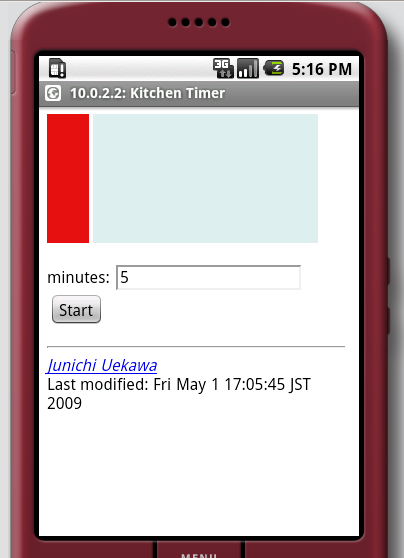
\includegraphics[width=0.3\hsize]{image200905/android-timer.png}

\subsection{Android$B$N4JC1$J%"%W%j%1!<%7%g%s$r:n@.$7$F5/F0$7$F$_$k(B}

$B$=$l$G$O!"(BAndroid $BMQ$N4JC1$J%"%W%j%1!<%7%g%s$r=q$$$F$_$^$7$g$&!#(B

\url{http://developer.android.com/guide/developing/eclipse-adt.html}
$B$K$7$?$,$C$FC8!9$H:n@.$7$^$9!#(B
$B$^$:!"(B
File$B$N(BNew Project $B$G(B Android $B$N$r%W%m%8%'%/%HA*Br$7$F:n@.$7$^$7$?!#(B
$B%?!<%2%C%H%S%k%I$O(B1.1$B$K$H$j$"$($:$7$m$H=q$$$F$"$j$^$9$,!"$h$/$o$+$i$J$$(B
$B$N$G!"<j85$N%U%!!<%`%&%'%"$N%P!<%8%g%s(B 1.5 $B$K$"$o$;$F$*$-$^$7$?!#(B

Run$B$N(BRun(Ctrl-F11)$B$G(BAndroid Application$B$rA*Br$9$k$H%(%_%e%l!<%?$r5/F0$7(B
$B$F%"%W%j%1!<%7%g%s$r<B9T$9$k$3$H$,$G$-$^$9!#(B
$B:G=i$K@8@.$5$l$?%=!<%9%3!<%I$N$^$^$N>uBV$@$H(B Hello World $B%"%W%j%1!<%7%g(B
$B%s$,5/F0$7$^$9!#(B

\subsection{Android$B$N4JC1$J%"%W%j%1!<%7%g%s$r=q$$$F$_$k(B}

$B%"%W%j%1!<%7%g%s$N:n@.$d%(%G%#%?$N5/F0$NItJ,$O$J$s$H$+$J$k$h$&$K$J$C$?$N(B
$B$G!"<!$O%A%e!<%H%j%"%k$rD/$a$F$_$^$9!#(B
Hello World$B$"$?$j$,$h$5$2$G$9!#(B

\url{http://developer.android.com/guide/tutorials/hello-world.html}

$B0lDL$jFI$s$G!"$H$j$"$($:%5%s%W%k$rD/$a$F$I$&$d$l$PJ8;zNs$rI=<($G$-$k$N$+(B
$B$r3NG'$7$?$N$G!"9%$-$JJ8;zNs$rI=<($9$k%"%W%j%1!<%7%g%s$r:n$C$F$_$^$9!#(B

Android $B$N(B top $B%3%^%s%I$G%W%m%;%9$N0lMw$r=PNO$G$-$k$N$G!"(B
$B%3%^%s%I$r<B9T$7$F$=$N=PNO$rI=<($9$k$@$1$N%"%W%j%1!<%7%g%s$r:n@.$7$F$_$^(B
$B$7$?!#(B
$BCf3K$r$J$9(Bsrc/jp.gr.netfort.dancer/TopView.java$B$O0J2<$N$h$&$K$J$j$^$7$?!#(B

\begin{commandline}
package jp.gr.netfort.dancer;

import android.app.Activity;
import android.os.Bundle;
import android.widget.TextView;
import java.io.*;

public class TopView extends Activity {
	/** Called when the activity is first created. */
	@Override
	public void onCreate(Bundle savedInstanceState) {
		super.onCreate(savedInstanceState);
		setContentView(R.layout.main);
		String [] command = { "top", "-n", "1"};
		String output = "";

		Runtime runtime = Runtime.getRuntime();
		Process process = null;
		try { 
			process = runtime.exec(command);
		} catch (Exception exception){
			System.exit(1);
		}
		BufferedReader reader = new BufferedReader(new InputStreamReader(process.getInputStream()));
		String line;
		try {
			while((line = reader.readLine()) != null) {
				output = output + line + "\n";
			}
		} catch (Exception exception) {
			System.exit(1);
		} finally {
			try {
				reader.close();
			} catch (Exception exception) {
				System.exit(1);
			}
		}
		TextView tv = new TextView(this);
		tv.setText(output);
		setContentView(tv);
	}
} 
\end{commandline}

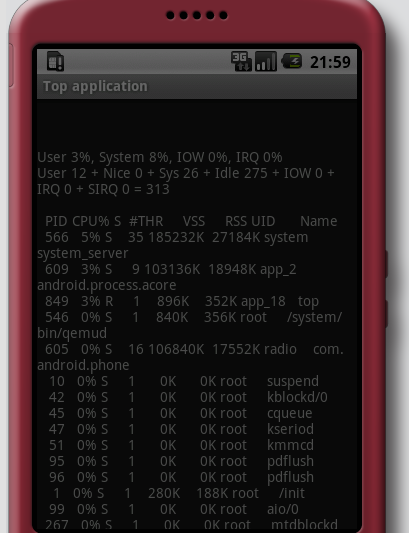
\includegraphics[width=0.3\hsize]{image200905/android-top.png}

\subsection{Android$B$N4JC1$J%"%W%j%1!<%7%g%s$r<B5!$G2TF/$5$;$F$_$k(B}

$B<B:]$K;H$&JXMx$J%"%W%j%1!<%7%g%s$r:n$C$F$_$^$7$g$&!#(B
$B%i%$%H%K%s%0%H!<%/$r<B;\$9$k:]$K$I$N%W%l%<%s%F!<%7%g%s$,5$$KF~$C$?$+$rI=(B
$BL@$9$k!"EjI<MQ$KMxMQ$9$k%\%?%s$G$b:n@.$7$^$7$g$&$+!#(B

\subsubsection{$B%(%U%'%/%HMQ$N%G!<%?(B}

$B$^$:!"$J$s$i$+$N8z2L2;$,I,MW$G$9!#(B
$B0JA0:n@.$7$?(Bding.wav $B$r$R$m$C$F$-$^$9!#(B
res/raw $B0J2<$K(B nautilus $B$+$i%I%i%C%0%"%s%I%I%m%C%W$G%3%T!<$7$^$9!#(B

$B$"$H!"%\%?%sIwL#$N2hA|$,I,MW$G$9!#(B
$BE,Ev$K(Bgimp$B$G3($r$+$$$F(B png $B%U%!%$%k$r:n@.$7$^$7$?!#(B

nautilus $B$+$i(B res/drawable $B0J2<$K(B png $B%U%!%$%k$r%I%i%C%0%"%s%I%I%m%C%W$G(B
$B%3%T!<$7$^$9!#(B

$B%U%!%$%kL>$+$i$=$N$^$^%j%=!<%9$NL>A0$r:n@.$9$k$?$a!"(B-$B$OMxMQ$G$-$J$$$h$&(B
$B$G$9!"(B \_ $B$OMxMQ$G$-$k$h$&$G$9!#:G=i(B he-up.png $B$r:n@.$7$h$&$H$7$F!"%(%i!<(B
$B$,=P$?$N$G(B he\_up.png $B$KJQ99$7$^$7$?!#(B

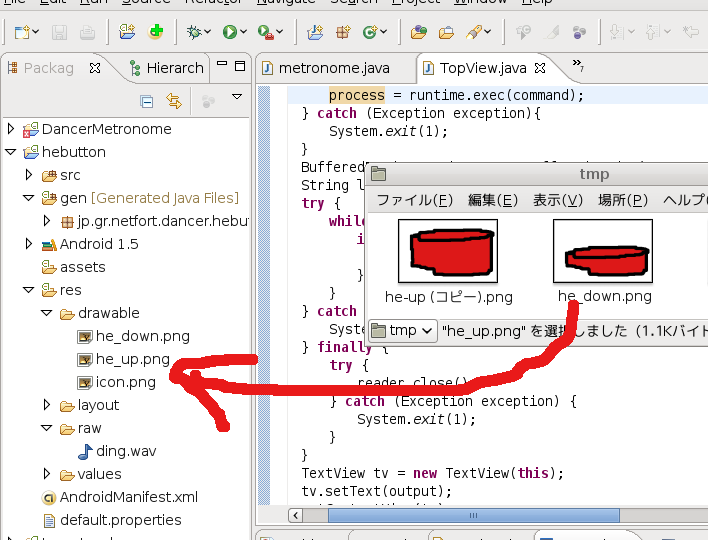
\includegraphics[width=0.5\hsize]{image200905/dragdrop.png}

\subsubsection{$B%l%$%"%&%H$N:n@.(B}

$B$*$b$`$m$K(B ImageButton $B$r:n@.$7$F!"(Bsrc$B$K2hA|%j%=!<%9$rDI2C$7$F$*$-$^$7$g(B
$B$&!#(B

\subsubsection{$B%/%j%C%/%"%/%7%g%s$N:n@.(B}

R.id.ImageButton01$B$KBP$7$F(B onClickListener$B$r:n@.$7!"%/%j%C%/$5$l$?=V4V$N(B
$BH?1~$r:n@.$7$^$7$g$&!#(B

$B2hA|$r%/%j%C%/$5$l$?>uBV$K@Z$jBX$($k$K$O(BImageButton$B$N(BsetImageResource()
$B$r8F$S=P$;$P$h$$$h$&$G$9!#(B

$B2;$r=P$9$K$O!"(BMediaPlayer $B$N%$%s%9%?%s%9$r:n@.$7!"(Bstart()$B$r8F$S=P$;$P$h(B
$B$$$h$&$G$9!#(B

$B0lDj;~4V7P2a$7$F$+$i85$N2hA|$KLa$9$K$O!"%"%i!<%`$r@_Dj$7$F%3!<%k%P%C%/$7(B
$B$F$b$i$($k$h$&$K$7$F!"%3!<%k%P%C%/$r8F$S=P$5$l$?$H$-$K=hM}$r$9$k$h$&$K$9(B
$B$l$P$h$$$h$&$G$9!#(B

\subsubsection{$B%5!<%PB&$N%"%/%7%g%s(B}

$B$=$l$G$O!"%/%j%C%/$5$l$?$H$-$K$I$&$$$&$3$H$r9T$&$N$+$N%"%/%7%g%s$r:n@.$7(B
$B$F$_$^$7$g$&!#(BHTTP$B%5!<%P$r=`Hw$7$^$9!#$3$&$$$&%$%m%b%N7O$N%5!<%P$r:n@.$9(B
$B$k$H$-$K$O(Bupaccho2 $B%5!<%P$r;H$&$3$H$,>e@n2H$N>o<1$J$N$G!"$=$l$rF'=1$7$^(B
$B$9!#(B($BM=Dj(B)

\subsection{$B$*$^$1(B:$B3+H/4D6-$KI,MW$J%a%b%j>CHq$O@a8:$G$-$k$N$+(B?}

$B<j85$N(BMacBook$B$K$O(B1GB$B$7$+%a%b%j$rEk:\$7$F$$$J$$$G$9!#(B
eclipse $B$O%G%U%)%k%H$N@_Dj$@$H5/F0$7$?=V4V$K(B1GB$B6a$/$N(B
$B2>A[%a%b%j$r>CHq$7!"B((BSwap$B$r;HMQ$7$F$7$^$&$H$$$&LdBj$,$"$j$^$7$?!#(B

\begin{commandline}
  PID USER      PR  NI  VIRT  RES  SHR S %CPU %MEM    TIME+  COMMAND            
17124 dancer    20   0  972m 302m  20m S    1 31.2   0:39.85 java
\end{commandline}

$B$H$j$"$($:!"%R%s%H$r5a$a$F(Bmaps$B$"$?$j$rD/$a$F$_$^$9!#(B
$B$=$l$J$j$K$?$/$5$s(Bmmap$B$7$F$$$^$9$,!"$=$l$@$1$G$O@bL@$G$-$J$$$h$&$J%a%b%j(B
$BNN0h$r3NJ]$7$F$$$^$9!#(B
\begin{commandline}
$ cat /proc/17124/status | grep Vm
VmPeak:	 1056748 kB
VmSize:	 1003316 kB
VmLck:	       0 kB
VmHWM:	  310740 kB
VmRSS:	  221616 kB
VmData:	  788504 kB
VmStk:	      84 kB
VmExe:	      36 kB
VmLib:	   38812 kB
VmPTE:	    1108 kB
$ cat /proc/17124/maps | grep rw | sort -rn -k5 
 .
\end{commandline}

$B$H$j$"$($:(BJava$B$N%"%W%j%1!<%7%g%s$N(BHeap$B$N;H$$J}$,$h$/$o$+$i$J$$$N$G!"(B
jconsole $B$G@\B3$7$FLdBj$r2r@O$7$^$9!#(B

$B%a%b%j%W!<%k$,$$$/$D$+$"$k$3$H$,$o$+$j$^$9!#(B

\begin{itemize}
 \item  Tenured Gen $B$,(B 60MB
 \item  Survivor 1MB
 \item  Code Cache $B$,(B 4MB
 \item  Perm Gen $B$,(B 70-90MB
 \item  Heap$B$O(B100MB(GC$B$7$?$i(B50MB$BDxEY(B)
\end{itemize}

eclipse.ini$B$,8=>u$3$&$J$C$F$$$k$N$G$9$,!"$3$l$r$*$=$k$*$=$k%A%e!<%K%s%0$7$F$_$^$9!#(B
\begin{commandline}
-showsplash
org.eclipse.platform
-framework
plugins/org.eclipse.osgi_3.4.2.R34x_v20080826-1230.jar
-vmargs
-Dosgi.requiredJavaVersion=1.5
-Xms40m
-Xmx256m
-XX:MaxPermSize=256m
\end{commandline}

$B5/F0;~$K3NJ]$7$?%R!<%W%a%b%j$NNN0h$r3+J|$7$F$$$J$$ItJ,$K$D$$$F$O!"(BGC$B$rIQ(B
$BHK$K9T$($P5/F0$O<c43CY$/$J$j$^$9$,$&$^$/$$$1$k$h$&$J5$$,$7$^$9!#(B
Xmx 128m$B$KJQ99$7$F$_$k$H!"<c43%a%b%j$N>CHq$,2<$,$j$^$7$?!#(B
$B$7$+$7$=$3$^$G7`E*$G$O$"$j$^$;$s$M!#(B
MaxPermSize$B$r(B64MB$B$K$9$k$H%(%i!<(B
\begin{commandline}
 Exception in thread "RMI TCP Connection(idle)" java.lang.OutOfMemoryError: PermGen space
\end{commandline}
$B$,H/@8$7$^$7$?!#(B
96MB$B$@$H%(%i!<$G$*$A$J$$$h$&$G$9!#(B

\begin{commandline}
  PID USER      PR  NI  VIRT  RES  SHR S %CPU %MEM    TIME+  $B%3%a%s%H(B
17124 dancer    20   0  972m 302m  20m S    1 31.2   0:39.85 java
19663 dancer    20   0  795m 296m  23m S    1 30.6   0:36.69 Heap 128MB$BHG(B
20266 dancer    20   0  661m 292m  22m S    1 30.1   0:41.62 MaxPermSize 96MB               
\end{commandline}

$B$,$s$P$C$F$_$?3d$K$O%a%b%j$,(B10MB$BDxEY$7$+@aLs$G$-$^$;$s$G$7$?!#%(%_%e%l!<(B
$B%?$b5/F0$7$F$$$k$H(B500MB$B$/$i$$(Bswap$B$K$$$C$F$7$^$&$N$G!"$D$i$$$G$9!#$7$+$b!"(B
$B%.%j%.%j$N%a%b%j@_Dj$K$7$F$$$?$H$3$m!"$$$m$$$m$HA`:n$7$F$$$k$H%a%b%j$,B-(B
$B$j$J$$$H$$$&%(%i!<$GMn$A$^$7$?!#$3$j$c%@%a$@!#%a%b%jGc$$$K$$$/$+$J!#(B

\begin{commandline}
-showsplash
org.eclipse.platform
-framework
plugins/org.eclipse.osgi_3.4.2.R34x_v20080826-1230.jar
-vmargs
-Dosgi.requiredJavaVersion=1.5
-Xms40m
-Xmx128m
-XX:MaxPermSize=96m
\end{commandline}

\subsection{$B;29MJ88%(B}

$BK\5-;v$N:n@.$K;29M$K$7$?J88%$G$9!#(B

\begin{itemize}
 \item \url{http://www.eclipse.org/}: eclipse
 \item \url{http://developer.android.com/}: Android $B$N%Z!<%8!"3+H/>pJs$,(B
       $B$^$H$^$C$F$$$k!#FC$K(B\url{http://developer.android.com/sdk/1.5_r1/index.html}: Android
       SDK 1.5$B$N%@%&%s%m!<%I%Z!<%8$+$i$?$I$k%Z!<%8$,=EMW!#(B
 \item
      \url{http://developer.android.com/guide/basics/what-is-android.html}: 
      SDK$B$N3+H/%^%K%e%"%k!#(B
      SDK $B$N(B\url{./android-sdk-linux_x86-1.5_r1/docs/}$B$KF1$8$b$N$,$"$k$N(B
      $B$G%*%U%i%$%s$G$b0B?4!#(B
      $B$?$@$7%*%s%i%$%s$N%I%-%e%a%s%H$OHyL/$JD{@5$,%"%C%W%G!<%H$5$lB3$1$F(B
      $B$$$k$h$&$J$N$G%M%C%H%o!<%/@\B3$,MxMQ$G$-$k%*%s%i%$%s$N>l9g$O$=$A$i(B
      $B$r;2>H$9$k$[$&$,$h$$$+$b$7$l$^$;$s!#(B
\end{itemize}

% ===============================================================
\dancersection{DDTSS$B3hMQ(B}{$B>e@n(B $B=c0l(B}
\index{ddtss2009}
% ===============================================================

\subsection{$B$O$8$a$K(B}

$B:G6a(B apt $B$N9q:]2=$b?J$_!"(BDebian archive $B$N(BDescription$B$NK]Lu$b%Q%C%1!<%8(B
$B$NG[I[$N;EAH$_$H0l=o$KG[I[$5$l$k$h$&$K$J$C$F$-$^$7$?!#(B
$B0lJ}!"K]Lu$rMQ0U$9$k%W%m%8%'%/%H(B(DDTP:Debian Description Translation
Project)$B$O$^$@Ia5Z$7$F$$$^$;$s!#(B
$B:#2s$O$=$N3hMQ$r;vA02]Bj$H$7$F!":#8e$I$&$d$C$F$&$^$/3hMQ$7$F$$$/$N$+$r9M(B
$B$($^$9!#(B

\subsection{Debian$B$N%Q%C%1!<%8@bL@J8$NK]Lu$NL\E*$H$O(B}

Debian Distribution$B$K$O?tK|$N%Q%C%1!<%8$,$"$j$^$9!#(B
$B%Q%C%1!<%8$N@bL@J8$O%$%s%9%H!<%k$9$k%=%U%H%&%'%"$rC5$9$N$K4sM?$9$kFbMF$G$"$kI,MW$,$"$j$^$9!#(B

$B8=:_!"$=$N@bL@J8$O$9$Y$F1Q(B
$B8l$GDs6!$5$l$F$$$^$9!#(B
$B$7$+$7!"1Q8l$G5-=R$5$l$F$$$k$H$=$b$=$b1Q8l$rM}2r$7$F$$$J$$$H$o$+$i$J$$It(B
$BJ,$,$"$j!"$7$+$b5;=QE*$J@lLgMQ8l$r$^$8$($?@bL@J8>O$OF|K\8l$r<g8@8l$H$9$k(B
$B%f!<%6$K$H$C$FM}2r$7$K$/$$>l9g$,$"$j$^$9!#(B

$B$=$b$=$b$N(BDescription$B$,K]Lu$KE,$9$k%l%Y%k$K;j$C$F$$$J$$!"F|K\8l$KLu$7$K$/(B
$B$$J8>O$G$"$l$P!"$b$H$NJ8=q$rD{@5$9$k$h$&$K0MMj$7$^$7$g$&!#(B

$B$^$?!"K]Lu$7$?(BDescription$B$,F|K\8l$H$7$FM}2r$7$K$/$$!"5;=QE*$JI=8=$,ITE,@Z$JI=8=$G$"$l$P!"$=$N(B
Description$B$OE,@Z$G$O$J$$$G$7$g$&!#(B

$B$^$?!"(BDebian$BA4BN$GI=5-$r$G$-$k$@$1E}0l$7$^$7$g$&!#F1$8FbMF$r@bL@$9$k$N$K(B
$BI=5-$N$f$l$,$"$k$H%Q%C%1!<%8$N@bL@J8$r$_$F$$$k$H$-$K$=$N:90[$KL\$,$$$C$F(B
$B$7$^$$$^$9!#(B

$B$=$NB>$K9MN8$9$kE@$O(B?

\subsection{DDTP}

DDTP $B$N@bL@$O(B Debian.org $B$N%Z!<%8$K$"$j$^$9(B: 
\url{http://www.debian.org/intl/l10n/ddtp.ja.html}$B!#(B
\url{http://www.debian.or.jp/community/translate/description-ja.html}
$B$J$I$H$"$o$;$FD/$a$F$/$@$5$$!#(B

$B%a!<%k%U%m%s%H%(%s%I$d!"%&%'%V%U%m%s%H%(%s%I$J$I$,$"$j$^$9!#(B

\subsection{DDTSS$B$H$O(B}

DDTP$B$N%U%m%s%H%(%s%I$N0l$D$,(BDDTSS$B$G$9!#(B
\url{http://ddtp.debian.net/ddtss/index.cgi/xx}
$B$KDs6!$5$l$F$$$^$9!#(B

\subsection{DDTSS$B3hMQ$N<j=g(B}

\subsubsection{$B%"%+%&%s%H$NEPO?(B}

$B%m%0%$%s2hLL(B\footnote{\url{https://ddtp.debian.net/ddtss/index.cgi/login}}$B$KHt$V$H!"(B
$B%"%+%&%s%H$r:n@.$9$k$?$a$N%j%s%/(B(Create$B!!(B
Login\footnote{\url{https://ddtp.debian.net/ddtss/index.cgi/createlogin}})
$B$,$"$k$N$G!"$=$3$+$i%"%+%&%s%HEPO?$7$^$9!#(B

$B%a!<%k$,FO$/$N$G!"$=$3$+$i%j%s%/$r%/%j%C%/$7$F%"%+%&%s%H$r%"%/%F%#%Y!<%H(B
$B$9$k$H!"%m%0%$%s2hLL$+$i%m%0%$%s$G$-$k$h$&$K$J$j$^$9!#(B

\subsubsection{$B%Q%C%1!<%8@bL@J8$NK]Lu:n@.(B}

\url{http://ddtp.debian.net/ddtss/index.cgi/ja}$B2hLL$G!"(B
Pending Translation $B$NMs$K$"$k%Q%C%1!<%8$rE,Ev$K%/%j%C%/$9$k$H!"%Q%C%1!<(B
$B%8@bL@J8$NJT=82hLL$,EP>l$7$^$9!#(B
$B0lIt$NJ8=q$,K]Lu$5$l$F$*$i$:(B\verb!<trans>!$B$H$J$C$F$$$?$j!"$^$C$?$/K]Lu$5(B
$B$l$F$$$J$+$C$?$j!"(B
$B>uBV$O$^$A$^$A$G$9!#(B

$B$3$N2hLL$GK]Lu$r:n@.$7$^$9!#(B

\subsubsection{$B%l%S%e!<$N<B;\(B}

\url{http://ddtp.debian.net/ddtss/index.cgi/ja}$B2hLL$G!"(B
Pending Review $B$NMs$K$"$k%Q%C%1!<%8$rE,Ev$K%/%j%C%/$9$k$H!"%Q%C%1!<%8@b(B
$BL@J8$N%l%S%e!<2hLL$,EP>l$7$^$9!#(B

$B%l%S%e!<$7$FJQ$JItJ,$,$"$l$PD{@5$7$^$7$g$&!#(B

\subsubsection{debian-doc$B%a!<%j%s%0%j%9%H$G$N%l%S%e!<<B;\(B}

debian-doc$B$H$$$&%a!<%j%s%0%j%9%H$G5DO@$H$+%l%S%e!<$O$*$3$J$&$_$?$$$G$9!#(B

\subsection{$B;29MJ88%(B}

$B0J2<$N%Z!<%8$b;29M$K$7$F$/$@$5$$!#(B

\begin{itemize}
 \item Debian $B%Q%C%1!<%8$N@bL@J8$rF|K\8l$GFI$_$?$$(B! $B!A(BDDTP $B$X$N$*M6$$!A(B 
       \url{http://www.debian.or.jp/community/translate/description-ja.html}
 \item $BIpF#7r;V$5$s$N(Bblog$B$N!X(BDebian$B%I%-%e%a%s%HK]Lu<jB3$-!Y(B:
       \url{http://kmuto.jp/d/index.cgi/debian/debian-doc-procedure.htm}
 \item $B>.NS576)$5$s$N(BDebian$BJY6/2q(B2006$BG/(B9$B7n;qNA!VK]Lu$X$NM6$$!W(B:
       \url{tokyodebian.alioth.debian.org/pdf/debianmeetingresume200609.pdf}
 \item debian-doc $B%a!<%j%s%0%j%9%H(B:
       $B<gMW$J5DO@$,9T$o$l$F$$$^$9!#<ALd$J$I$b!"$3$A$i$G!#(B
\end{itemize}


\clearpage

%\printindex

\cleartooddpage

\vspace*{15cm}
\hrule
\vspace{2mm}

\includegraphics[width=2cm]{image200502/openlogo-nd.eps}
\noindent \Large \bf Debian $BJY6/2q;qNA(B\\ \\
\noindent \normalfont \debmtgyear{}$BG/(B\debmtgmonth{}$B7n(B\debmtgdate{}$BF|(B \hspace{5mm}  $B=iHGBh(B1$B:~H/9T(B\\
\noindent \normalfont $BEl5~%(%j%"(B Debian $BJY6/2q(B $B!JJT=8!&0u:~!&H/9T!K(B\\
\hrule


\end{document}
